\documentclass[a4paper,10pt]{article}

\usepackage{bm}
\usepackage{url}
\usepackage{bera}
\usepackage{epsfig}
\usepackage{comment} 
\usepackage{amsmath}
\usepackage{amssymb}
\usepackage{amsfonts}
\usepackage{hyperref}
\usepackage{listings}
\usepackage[T1]{fontenc}
\usepackage[margin=1.0in]{geometry}
\usepackage[square, comma, numbers, sort&compress]{natbib}

%opening
\title{Eigenstate Thermalization in Drive-Quenched Quantum Systems}
\author{Analabha Roy, Arti Garg \\
\textit{TCMP division, Saha Institute of Nuclear Physics,}\\ 
\textit{Kolkata, India}}

\begin{document}

\maketitle
\section{\sc Introduction}
In this work, we seek to contribute to recent discussions on the general relation between integrability and thermalization in the nonequilibrium dynamics of quantum many body systems. The most basic nonequilibrium process that is experimentally viable in quantum gases of ultracold atoms is the \textit{quantum quench}. Here, one of the confining parameters of the system is changed abruptly, either as a Heaviside impulse or with a known time dependence, following which the state of the system is allowed to evolve dynamically according to the Schr\"odinger equation. Recent studies have shown that that the long-time asymptotic behavior of a quantum system out of equilibrium is dependent on its integrability. Nonintegrable systems have been seen to \textit{thermalize}, where time averages of dynamical observables do not depend on the initial conditions~\cite{deutsch,olshanii:ipr, rigol:nature, krishnenduda:ethreview}, but only on the initial energy. Such 'thermal' behavior cannot, in general, be seen in integrable systems, where additional initial state information is required in order to predict the dynamical steady state. Such informations are embedded in constants of motion that form the \textit{Generalized Gibbs Ensemble} via Lagrange multipliers. Other predictions have centered around claims that even integrable models can show some thermal characteristics, such as an effective temperature that depends only on the initial energy. Small quenches reportedly show relaxation time scales consistent with thermal equilibrium at a finite temperature~\cite{leticia,rossini}.

Following references~\cite{rossini,leticia}, we are going to investigate the possibility that a $1$D reduced BCS model with chemical potential $\Gamma$, that can be mapped to the spin-$1/2$ quantum Ising model in a transverse magnetic field $\Gamma$, can show thermal-like behavior after various types of quantum quenches. We start with different types of impulse quenches, and then move on to periodic drives and then to combinations of impulse quenches modulated by resonant periodic drives. The idea is to compare the energy associated with the initial state to the average energy of a \textit{fictitious} thermal state at an effective temperature $\beta=(k_bT)^{-1}$ in an effective grand canonical ensemble. The dynamics can be predicted independently due to the integrable nature of the system, allowing us to determine the extent of thermalization in a response quantity like magnetization by comparing the time average of the same with the statistical average over the fictitious ensemble at temperature $T$. The evolution of a quantum system with Hamiltonian $\mathrm{H}$ is given by the many body state $|\Psi(t)\rangle$, which can be obtained by solving the Schr\"odinger equation,
\begin{equation}
 \label{eq:schr:mb}
 \mathrm{H}|\Psi(t)\rangle = i\frac{\partial}{\partial t}|\Psi(t)\rangle,
\end{equation}
for integrable systems. Like all first order differential equations, the solution requires knowledge of the initial state $|\Psi_0\rangle=|\Psi(t=0)\rangle$. A time independent $\mathrm{H}$ keeps the total energy conserved at $E_0=\langle\Psi_0|\mathrm{H}|\Psi_0\rangle$, at all times. The question here is, can the asymptotic state of the system be described, in whole or in part, by a density matrix $\rho$ that maximizes the informational entropy functional $S[\rho_c]=-\mbox{Tr}[\rho_c\ln{\rho_c}]$, where the subscript $c$ denotes the constraint 
that keeps the energy conserved at $E_0$ ? The constraint can be rewritten as
\begin{equation}
\label{eq:enconstr}
\langle\Psi_0|\mathrm{H}|\Psi_0\rangle = \frac{\mbox{Tr}[e^{\beta\mathrm{H}}\mathrm{H}]}{\mbox{Tr}[e^{\beta\mathrm{H}}]}.
\end{equation}
The thermalization question attempts to relate the time average and/or asymptotic behavior of a response quantity $\overline{\langle\mathcal{O}(t)\rangle}$ from an observable $\mathcal{O}$ (where the overline denotes time average and $\langle\cdots\rangle$ denotes the quantum expectation value) to the thermal average of the fictitious ensemble \textit{i.e.} ${\mbox{Tr}[e^{\beta\mathrm{H}}\mathcal{O}]}/{\mbox{Tr}[e^{\beta\mathrm{H}}]}$. For the Ising chain, the dynamical expectation value can be decomposed to a sum over different modes in disjoint Hilbert subspaces, and thermal behavior should lead to a $\beta$ that is the same for all modes. This does not always happen in integrable systems, although mode-dependent $\beta$s can be obtained~\cite{krishnenduda:ethreview}. In addition, such an effective thermal distribution is expected to be independent of the nature of the quench and the initial conditions. However, the analysis below shows this to not be the case, leading us to delve deeper into alternative descriptions of temperature and thermalization as detailed in~\cite{leticia}.

\section{\sc Model and Dynamics}
\label{sec:tls}
Our starting Hamiltonian is written in units of the tight-binding hopping amplitude in a $1$ dimensional lattice as
\begin{equation}
\label{eq:hamiltonian}
\mathrm{H} = -\sum_i \left[c^\dagger_ic^{ }_{i+1} + \alpha c^\dagger_ic^\dagger_{i+1}+h.c.\right]-\Gamma\sum_i\left(1-2c^\dagger_ic^{ }_i\right),
\end{equation}
where the tight-binding approximation has been made for the kinetic energy. Also, $-2\Gamma$ is the chemical potential, and $\alpha$ is a source term which contributes to the gap~\cite{arti:garg}. This Hamiltonian can be mapped into an $SU(2)$ representation in the reciprocal lattice space using Nambu spinors $( c^\dagger_k , c_{-k})$ to get
\begin{equation}
\label{eq:hamiltonian:su2}
\mathrm{H}=\sum^N_{k\in\mathcal{W}} \begin{pmatrix}
                   c^\dagger_k & c_{-k}
                  \end{pmatrix}
		 \mathrm{H}_k
		  \begin{pmatrix}
                           c_k \\
			   c^\dagger_{-k}
                          \end{pmatrix},
\end{equation}
where the Hamiltonian
\begin{equation}
\label{eq:hk}
\mathrm{H}_k =  \begin{bmatrix}
		  \Gamma-\cos{k} & i\alpha \sin{k} \\
		  -i\alpha \sin{k} & -\Gamma+\cos{k}
		  \end{bmatrix}=\left(\Gamma-\cos{k}\right)\sigma_z-\left(\alpha\sin{k}\right)\sigma_y.
\end{equation}
Also, $k$ is the crystal momentum that lies inside the First Brillouin Zone $\mathcal{W}=[-\pi,\pi]$, and $N$ is the number of lattice sites. The state  of this system is denoted by $|\Psi(t)\rangle\equiv\prod_{k\in\mathcal{W}}|\psi_k(t)\rangle$, where $|\psi_{k}(t)\rangle = \left[u_{k}(t)-iv_{k}(t)c^\dagger_kc^\dagger_{-k}\right]|0\rangle$. Here, $u_k(t)$ and $v_k(t)$ are the particle and hole amplitudes respectively. The unperturbed eigensystem is 
\begin{equation}
\label{eq:unpert:esystem}
H_k:\bigg\{\begin{array}{ll}
           +E_k &;|\uparrow_k\rangle=\begin{pmatrix}
                                    +u_k\\
                                    -iv_k
                                   \end{pmatrix}\\
          -E_k &; |\downarrow_k\rangle = \begin{pmatrix}
                                           +v_k\\
                                           +iu_k
                                          \end{pmatrix}
           \end{array},
\end{equation}
where
\begin{eqnarray}
\label{eq:ukvk}
 u_k,(v_k) &\equiv& \sqrt{\frac{E_k+(-) f_k}{2E_k}},\nonumber \\
 E_k &\equiv& \sqrt{f^2_k+\Delta^2_k},\nonumber \\
 f_k &\equiv& \Gamma -\cos{k},\nonumber \\
 \Delta_k &\equiv& \alpha\sin{k}.
\end{eqnarray}
For all subsequent dynamics, we wish to start from this state at $t=0$. Thus, $u_k(0)=u_k$, and $v_k(0)=v_k$. The dynamics is solved by the Schr\"odinger equations
\begin{equation}
 \label{eq:schroedinger}
H_k|\psi_k(t)\rangle = i\frac{\partial}{\partial t}|\psi_k(t)\rangle \mbox{  } \forall k\in\mathcal{W}.
\end{equation}

\begin{comment}
\section{\sc Many Body Tower of States}
\label{sec:eth:micro}

\textbf{Warning: Old Notation}\\

The full many body Hamiltonian in eq~\ref{eq:hamiltonian:su2} is diagonalized by the Bogoliubov operators $\alpha_{k}=u_kc_k-iv_kc^\dagger_{-k}$, yielding $\mathrm{H}=\left(1/2\right)\sum^N_{k\in\mathcal{W}}E_k\left(\alpha^\dagger_k\alpha^{ }_k-\alpha^\dagger_{-k}\alpha^{ }_{-k}\right)$. The ground state, denoted by $|0\rangle_B$ as the vacuum of Bogoliubov excitations, is given by $|0\rangle_B=\prod^N_{p\in\mathcal{W}}\left[u_{p}-iv_{p}c^\dagger_pc^\dagger_{-p}\right]|0\rangle$ in the particle-hole basis. Its energy is given by $\mathcal{E}_0=-\sum^N_{p\in\mathcal{W}}E_p$. Its effective magnetization, the expectation value of $\sum^N_{p\in\mathcal{W}} \sigma^{(p)}_z$, is given by $\mathcal{Q}_0=\sum^N_{p\in\mathcal{W}}\left(1-2|v_p|^2\right)$. Thus, the tower of $2^N$ eigenstates will be given by
\begin{eqnarray}
\label{eq:towerofestates}
 |0\rangle_B & &, \nonumber \\  
 |k\rangle_B &=& \alpha^\dagger_k|0\rangle_B , \nonumber \\
 |k_1,k_2\rangle_B &=& \alpha^\dagger_{k_1}\alpha^\dagger_{k_2}|0\rangle_B ,\nonumber \\
 |k_1,k_2,k_3\rangle_B &=& \alpha^\dagger_{k_1}\alpha^\dagger_{k_2}\alpha^\dagger_{k_3}|0\rangle_B, \nonumber \\
            & &  \dots \nonumber \\
 |k_1,k_2,k_3 \dots k_m\rangle_B &=&  \alpha^\dagger_{k_1}\alpha^\dagger_{k_2}\alpha^\dagger_{k_3}\dots\alpha^\dagger_{k_m}|0\rangle_B, \nonumber \\
            & &  \dots  \nonumber \\
 |k_1,k_2,k_3 \dots k_N\rangle_B &=& \prod^N_{k\in\mathcal{W}}\alpha^\dagger_k|0\rangle_B.
\end{eqnarray}
Here, the first line represents the state of no excitations, the second line represents the $N$ single particle excitations, the third represents the $^NC_2$ two-particle excitations, the $(m+1)^{\rm th}$ line represents the $^NC_m$ $m$-particle excitations, and the final line represents the single state of all excitations. The energy eigenvalues of these states with respect to $\mathcal{E}_0$ are given by $\mathcal{E}_{k_1,k_2,k_3 \dots k_m}=\sum_{k_1 k_2 k_3\dots k_m}E_k$. The magnetization of each of these states with respect to $\mathcal{Q}_0$ are given by \newline $\mathcal{Q}_{k_1,k_2,k_3 \dots k_m}=\sum_{k_1 k_2 k_3\dots k_m}\left(1-2|v_k|^2\right)$. At $t=0-$, the system is populated in state $|\Psi_0\rangle$ that is decomposed in the Hamiltonian eigenbasis as
\begin{multline}
\label{eq:psi0:ebasis}
|\Psi_0\rangle=C_0|0\rangle_B+\sum_{k}C_k|k\rangle_B+\sum_{k_1 k_2}C_{k_1 k_2}|k_1,k_2\rangle_B \\
+\sum_{k_1 k_2 k_3}C_{k_1 k_2 k_3}|k_1,k_2,k_3\rangle_B+\dots+\sum_{k_1 k_2 k_3 \dots k_m}C_{k_1 k_2 k_3 \dots k_m} |k_1,k_2,k_3 \dots k_m\rangle_B+\dots\\
+\sum_{k_1 k_2 k_3 \dots k_N}C_{k_1 k_2 k_3 \dots k_N} |k_1,k_2,k_3 \dots k_N\rangle_B.
\end{multline}
The 'initial energy' of the state is defined to be~\cite{rigol:nature} $E_0=\langle\Psi_0|\mathrm{H}|\Psi_0\rangle=|C_0|^2\mathcal{E}_0+\sum_{k}|C_k|^2\mathcal{E}_k+\sum_{k_1 k_2}|C_{k_1k_2}|^2\mathcal{E}_{k_1 k_2}+
\sum_{k_1 k_2 k_3}|C_{k_1k_2k_3}|^2\mathcal{E}_{k_1k_2k_3}+
\dots+\sum_{k_1 k_2 k_3\dots k_m}|C_{k_1k_2k_3\dots k_m}|^2\mathcal{E}_{k_1k_2k_3\dots k_m}+\dots+|C_{k_1k_2k_3\dots k_N}|^2\mathcal{E}_{k_1k_2k_3\dots k_N}$. As the system evolves in time from $t=0+$ according to the Schr\"odinger equation, the time-average of observables like magnetization can be approximated by averaging out all destructive interferences~\cite{deutsch,rigol:nature}. Simplifying the solution $|\Psi(t)\rangle = \exp{\left(i\mathrm{H}t\right)}|\Psi_0\rangle$ in the Hamiltonian eigenbasis yields
\begin{multline}
\label{eq:fullstate}
|\Psi(t)\rangle=C_0|0\rangle_B e^{i\mathcal{E}_0 t}+\sum_{k}C_k|k\rangle_Be^{i\mathcal{E}_k t}+\sum_{k_1 k_2}C_{k_1 k_2}|k_1,k_2\rangle_B e^{i\mathcal{E}_{k_1k_2} t}\\
+\sum_{k_1 k_2 k_3}C_{k_1 k_2 k_3}|k_1,k_2,k_3\rangle_Be^{i\mathcal{E}_{k_1k_2k_3} t}+\dots+\sum_{k_1 k_2 k_3 \dots k_m}C_{k_1 k_2 k_3 \dots k_m} |k_1,k_2,k_3 \dots k_m\rangle_Be^{i\mathcal{E}_{k_1k_2k_3\dots k_m} t}+\dots\\
+\sum_{k_1 k_2 k_3 \dots k_N}C_{k_1 k_2 k_3 \dots k_N} |k_1,k_2,k_3 \dots k_N\rangle_Be^{i\mathcal{E}_{k_1 k_2 k_3 \dots k_m} t}.
\end{multline}
The time average of the magnetization is defined as 
\begin{equation}
Q\equiv  \lim_{T\rightarrow\infty}\frac{1}{T}\int^T_0\mathrm{d}t\quad\langle\Psi(t)|\sum_k\sigma^{(k)}_z|\Psi(t)\rangle.
\end{equation}
Using this and eqn~\ref{eq:fullstate}, we can average out all oscillatory terms to $0$, yielding
\begin{multline}
\label{eq:timeavq}
Q=|C_0|^2\mathcal{Q}_0+\sum_{k}|C_k|^2\mathcal{Q}_k+\sum_{k_1 k_2}|C_{k_1k_2}|^2\mathcal{Q}_{k_1 k_2}+
\sum_{k_1 k_2 k_3}|C_{k_1k_2k_3}|^2\mathcal{Q}_{k_1k_2k_3}+ \dots\\
+\sum_{k_1 k_2 k_3\dots k_m}|C_{k_1k_2k_3\dots k_m}|^2\mathcal{Q}_{k_1k_2k_3\dots k_m}+\dots+|C_{k_1k_2k_3\dots k_N}|^2\mathcal{E}_{k_1k_2k_3\dots k_N}.
\end{multline}
We now simplify these expressions by assigning a unique identifier $\gamma$ to each eigenstate of $k_1 k_2 k_3 \dots k_m$ set, say, an integer between $0$ and $2^N$. Thus, $|\Psi_0\rangle=\sum_\gamma C_\gamma |\gamma\rangle_B$, $E_0=\sum_\gamma |C_\gamma|^2 \mathcal{E}_\gamma$, and $Q=\sum_\gamma |C_\gamma|^2 \mathcal{Q}_\gamma$. 

\textbf{The Eigenstate Thermalization posits that physically meaningful choices of $|\Psi_0\rangle$} (for instance, the ground state of a many body Hamiltonian $\mathrm{H}'= \mathrm{H}-\delta\mathrm{H}$) \textbf{will produce a single global peak in the distribution of $|C_\gamma|^2$ as a function of $\gamma$. This peak value $\bar{\gamma}$ will have a spread in $|C_\gamma|^2$ of small width $2\delta\bar{\gamma}$ such that, in some 'nonintegrable limit',}
\begin{equation}
Q\approx\sum_{\bar{\gamma}-\delta\bar{\gamma}\leq \gamma\leq \bar{\gamma}+\delta\bar{\gamma}}\mathcal{Q}_\gamma,
\end{equation}
\textbf{and that , $\forall\gamma$ in the interval $\left[\bar{\gamma}-\delta\bar{\gamma},\bar{\gamma}+\delta\bar{\gamma}\right]$, the quantity $|E_0-N\mathcal{E}_\gamma|$ is bounded above by a quantity $\delta\mathcal{E}\ll N$}. Under such circumstances, the steady state of the system can be said to be 'thermalized' over a microcanonical ensemble of spanned by the $\gamma$s in the interval  $\left[\bar{\gamma}-\delta\bar{\gamma},\bar{\gamma}+\delta\bar{\gamma}\right]$, where the eigenstates inside the ensemble are all very close to the initial energy per particle. The 'nonintegrable limit' seems to mean that the system has fewer than $N$ nontrivial symmetries \textit{i.e} symmetries other than $\mathrm{H}^n$ or $\sum^n_{\gamma_i}|\gamma_i\rangle\langle\gamma_i|$ where $n\leq N$. An impulse quench, carried out instantaneously at $t=0$, can take the system from $\mathrm{H}-\delta\mathrm{H}$ to $\mathrm{H}$, and is expected to produce such a 'thermalized' steady state. The question that can be asked here is 
whether this process is dependent on the mechanism of the quench or not, and the detailed dynamics of a specific time dependent quench with periodic modulation can be used to investigate this.
\end{comment}

\section{\sc Thermalization with initial conditions}
We can now let the system evolve with different initial conditions to see if it settled down into a time-averaged state that can be described by thermal characteristics. Regardless of what initial conditions we choose, the system evolves in time with the time translation operator $\mathcal{U}(t)=\exp{\left[-i\mathrm{H}t\right]}$, obtained by solving the Schr\"odinger equation~\ref{eq:schroedinger}. We define the dynamical magnetization operator in the Heisenberg representation to be
\begin{equation}
\label{eq:mopdef}
\hat{m}(t) = \mathcal{U}^\dagger (t)\left[\sum_k\sigma^{(k)}_z\right] \mathcal{U}(t).
\end{equation}
The time-averaged dynamical magnetization can be obtained from the above expression as
\begin{eqnarray}
\label{eq:mdyn}
m_{dyn}&=&\overline{m(t)},\nonumber \\
m(t)   &=& \langle \Psi_0 |\hat{m}(t)|\Psi_0 \rangle \nonumber \\
       &=& \langle \Psi_0 |e^{-i\sum_p\mathrm{H}_p t}\left[\sum_k\sigma^{(k)}_z\right]e^{i\sum_p\mathrm{H}_p t}|\Psi_0\rangle \nonumber \\
       &=& \langle \Psi_0 |e^{-i\sum_p\mathrm{H}_p t}\left[\sum_k\sigma^{(k)}_z e^{i\mathrm{H}_k t} e^{i\sum_{p\neq k}\mathrm{H}_p t}\right]|\Psi_0\rangle \nonumber \\
       &=&\langle \Psi_0 |\left[\sum_k e^{-i\sum_{p\neq k}\mathrm{H}_p t}\otimes e^{-i\mathrm{H}_k t}\sigma^{(k)}_z e^{i\mathrm{H}_k t} \otimes e^{i\sum_{p\neq k}\mathrm{H}_p t}\right]|\Psi_0\rangle \nonumber \\
       &=& \langle \Psi_0 |\left[\sum_k e^{-i\sum_{p\neq k}\mathrm{H}_p t}e^{i\sum_{p\neq k}\mathrm{H}_p t}\otimes e^{-i\mathrm{H}_k t}\sigma^{(k)}_z e^{i\mathrm{H}_k t} \right]|\Psi_0\rangle \nonumber \\
       &=& \langle \Psi_0 |\left[\sum_k e^{-i\mathrm{H}_k t}\sigma^{(k)}_z e^{i\mathrm{H}_k t} \right]|\Psi_0\rangle.
\end{eqnarray}
where the overline indicates time average, and $|\Psi_0\rangle$ is the many-body state of the system at $t=0$. The operator
\begin{multline}
e^{-i\mathrm{H}_k t}\sigma_z e^{i\mathrm{H}_k t} =\alpha \sin{k}\left(\frac{\sin{2E_kt}}{E_k}\right)\sigma_x+
\alpha\left(\sin{2k}-2\Gamma\sin{k}\right)\left(\frac{\sin^2{2E_kt}}{E^2_k}\right)\sigma_y+\\
\bigg\{\cos^2{E_kt}+\left[\left(\Gamma-\cos{k}\right)^2-\alpha^2\sin^2{k}\right]\left(\frac{\sin^2{2E_kt}}{E^2_k}\right)\bigg\}\sigma_z
\end{multline}
where we have substituted the rhs of eq~\ref{eq:hk} for $\mathrm{H}_k$ and expanded the expressions using Pauli algebra. Now, the oscillatory terms can be averaged out and the expectation values of the Pauli matrices with respect to the initial state (denoted by $\langle\cdots\rangle$) added to yield
\begin{equation}
\label{eq:mop}
\langle\overline{e^{-i\mathrm{H}_k t}\sigma_z e^{i\mathrm{H}_k t}}\rangle =\frac{\alpha}{2E^2_k}\left(\sin{2k}-2\Gamma\sin{k}\right)\langle\sigma_y\rangle+\frac{1}{2}\bigg\{1+\left[\frac{\left(\Gamma-\cos{k}\right)^2-\alpha^2\sin^2{k}}{E^2_k}\right]\bigg\}\langle\sigma_z\rangle.
\end{equation}
Equations~\ref{eq:mop} and~\ref{eq:mdyn} can be used to calculate the time-averaged transverse magnetization of the system for a particular choice of initial state $|\Psi_0\rangle$. The idea is to compare this quantity to a thermalized magnetization in order to see if this steady state contains any ergodic or thermal information. 

The corresponding thermal magnetization must be obtained by choosing a suitable effective 'temperature' $\beta=(k_BT)^{-1}$. To do that, we first note that the thermal average of energy at temperature $\beta=(k_BT)^{-1}$ can be written in terms of the density matrix as $E_{th}=\mbox{Tr}[\mathrm{H} e^{\beta \mathrm{H}}]/\mbox{Tr}[e^{\beta \mathrm{H}}]$. Using equation~\ref{eq:hk}, this simplifies to $E_{th}=\mbox{Tr}[\sum_k \mathrm{H}_k e^{\beta \sum_k\mathrm{H}_k}]/\mbox{Tr}[e^{\beta \sum_k \mathrm{H}_k}]=(\partial/\partial\beta) \ln{\mbox{Tr}[e^{\beta \sum_k \mathrm{H}_k}]}$. The partition function $Z=\mbox{Tr}[e^{\beta \sum_k \mathrm{H}_k}]$ simplifies to $Z=\prod_k \mbox{Tr}[e^{\beta \mathrm{H}_k}]$, since the different $H_k$'s are over disjoint Hilbert subspaces. Thus, $\ln{Z}=\sum_k \ln{\mbox{Tr}[e^{\beta \mathrm{H}_k}]}=\sum_k\ln{[e^{\beta E_k}+e^{-\beta E_k}]}=\sum_k \ln{[2 \cosh{\beta E_k}]}$. Therefore, $E_{th}=\sum_k E_k \tanh{\beta E_k}$. Now, as the system evolves in time, its energy is preserved 
at the initial expectation value. Thus, the equivalent temperature of thermalization can be obtained by solving for $\beta$ from the equation
\begin{equation}
\label{eq:tempsolve}
\langle\Psi_0|\mathrm{H}|\Psi_0\rangle = \frac{\mathrm{N}}{2\pi}\int^{\pi}_{-\pi}\mathrm{d}k \quad E_k \tanh{\beta E_k},
\end{equation}
where the continuum limit has been taken. If there is any meaningful thermalization in the asymptotic limit, the equivalent thermal magnetization at this temperature must match the asymptotic or time-averaged behavior of the dynamical magnetization. The former is given by 
\begin{eqnarray}
 m_{th}&=& \frac{1}{Z}\times \mbox{Tr}[\sum_k\sigma_z e^{\beta \sum_p\mathrm{H}_p}]\nonumber \\
       &=& \sum_k \frac{\mbox{Tr}[\sigma_z e^{\beta H_k}]\times \prod_{p\neq k}\mbox{Tr}[e^{\beta \mathrm{H}_p}]}{\mbox{Tr}[e^{\beta \mathrm{H}_k}]\times\prod_{p\neq k}\mbox{Tr}[e^{\beta \mathrm{H}_p}]},\nonumber \\
       &=& \sum_k \frac{\mbox{Tr}[\sigma_z e^{\beta H_k}]}{\mbox{Tr}[e^{\beta \mathrm{H}_k}]},
\end{eqnarray}
where the second line in the equations above comes about as a result of the relation $\mbox{Tr}[e^{\beta (\mathrm{H}_{k_1}+\mathrm{H_{k_2}})}]=\mbox{Tr}[e^{\beta \mathrm{H}_{k_1}}]\times \mbox{Tr}[e^{\beta \mathrm{H}_{k_2}}]$ $\forall k_1, k_2$ on account of the different momenta spanning disjoint Hilbert spaces. Thus,
\begin{eqnarray}
\label{eq:mth}
 m_{th}&=& \sum_k \frac{\mbox{Tr}[\sigma_z e^{\beta H_k}]}{\mbox{Tr}[e^{\beta \mathrm{H}_k}]}\nonumber \\
       &=& \sum_k \frac{Tr\bigg\{\sigma_z e^{\beta\left[\left(\Gamma-\cos{k}\right)\sigma_z-\alpha\sin{k}\sigma_y\right]}\bigg\}}{2\cosh{\beta E_k}},\nonumber \\
       &=& \sum_k \left(1-2|v_k|^2\right)\tanh{\beta E_k},
\end{eqnarray}

Below, we choose three types of quantum quenches that lead to three distinct choices of the initial state.
\subsection{Vacuum state quench}
First, we choose the initial state to be the state of no particles, \textit{i.e} the vacuum. Physically, this problem would be equivalent to a diabatic quenched 'switching on' of the optical lattice. Also, this would correspond to a rapid quench in $\alpha$ from $0$ to its steady value for $\Gamma\geq1$, since the adiabatic ground state for $\alpha=0, \Gamma\geq 1$ is simply the vacuum. Thus, the initial state is $|\Psi_0\rangle = |0\rangle$, or
\begin{equation}
\label{eq:psi0}
|\Psi_0\rangle=\prod_q \left(u^0_q-iv^0_qc^\dagger_{q}c^\dagger_{-q}\right)|0\rangle,
\end{equation}
where the coefficients
\begin{equation}
\label{eq:icg}
u^0_q (v^0_q) = 1 (0) \forall q.
\end{equation}
\begin{comment}

\textbf{Warning:Old Notation}\\


Thus, using Eqns~\ref{eq:psi0:ebasis} and~\ref{eq:psi0}, as well as Eqn~\ref{eq:towerofestates} we get
\begin{eqnarray}
C_\gamma &=& \langle\gamma|\Psi_0\rangle \nonumber \\
         &=& _B\langle0|\alpha^{ }_{k_m} \alpha^{ }_{k_{m-1}}\dots \alpha^{ }_{k_2}\alpha^{ }_{k_1}\prod_q \left(u^0_q-iv^0_qc^\dagger_{q}c^\dagger_{-q}\right)|0\rangle \nonumber \\
         &=& \prod_{k\in\gamma}\left(v^{ }_ku^0_k-u^{ }_kv^0_k\right) \prod_{q\not\in\gamma}\left(u^{ }_qu^0_q+v^{ }_qv^0_q\right).
\end{eqnarray}
Here, $\gamma$ denotes a particular combination of $m$ sets of excited momenta $k_1\dots k_m$. 
\end{comment}
The 'energy' of the state $|\Psi_0\rangle$, relative to the ground state, is given by
\begin{eqnarray}
E_0 &=& \langle\Psi_0|\mathrm{H}|\Psi_0\rangle \nonumber \\
    &=& \sum_k\bigg\{\left(\Gamma-\cos{k}\right)\left[1-2(v^0_k)^2\right]-2\alpha u^0_kv^0_k\sin{k}\bigg\} \nonumber \\
    &=& N\Gamma,
\end{eqnarray}
assuming $\Gamma$ to always be nonegative. 
\begin{comment}

\textbf{Warning:Old Notation}\\


Thus, $C_\gamma=\prod_{k\in\gamma}v_k\prod_{q\not\in\gamma}u_q$. Note that, even with nonzero $\Gamma$, $u_k,v_k$, are very much like mutually reflected step functions provided $\Gamma$ is very small. Thus, $C_\gamma$ is expected to be almost zero for most values of $\gamma$, and sharply peaked at near-unity values for a small number of $\gamma$s (say, ${\gamma}'$). Thus, we can approximate the time average of the magnetization from Eq.~\ref{eq:timeavq} as $Q\approx\sum_{\gamma'}\mathcal{Q}_{\gamma'}$. 
All of the above can be simplified by the following equivalent formalism. 
\end{comment}
The equivalent temperature of thermalization can be obtained by solving for $\beta$ from the eq~\ref{eq:tempsolve} to yield
\begin{equation}
\label{eq:tempsolve1}
\Gamma\pi = \int^{\pi}_{0}\mathrm{d}k \quad E_k \tanh{\beta E_k},
\end{equation}
\begin{figure}[h!bt]
\ 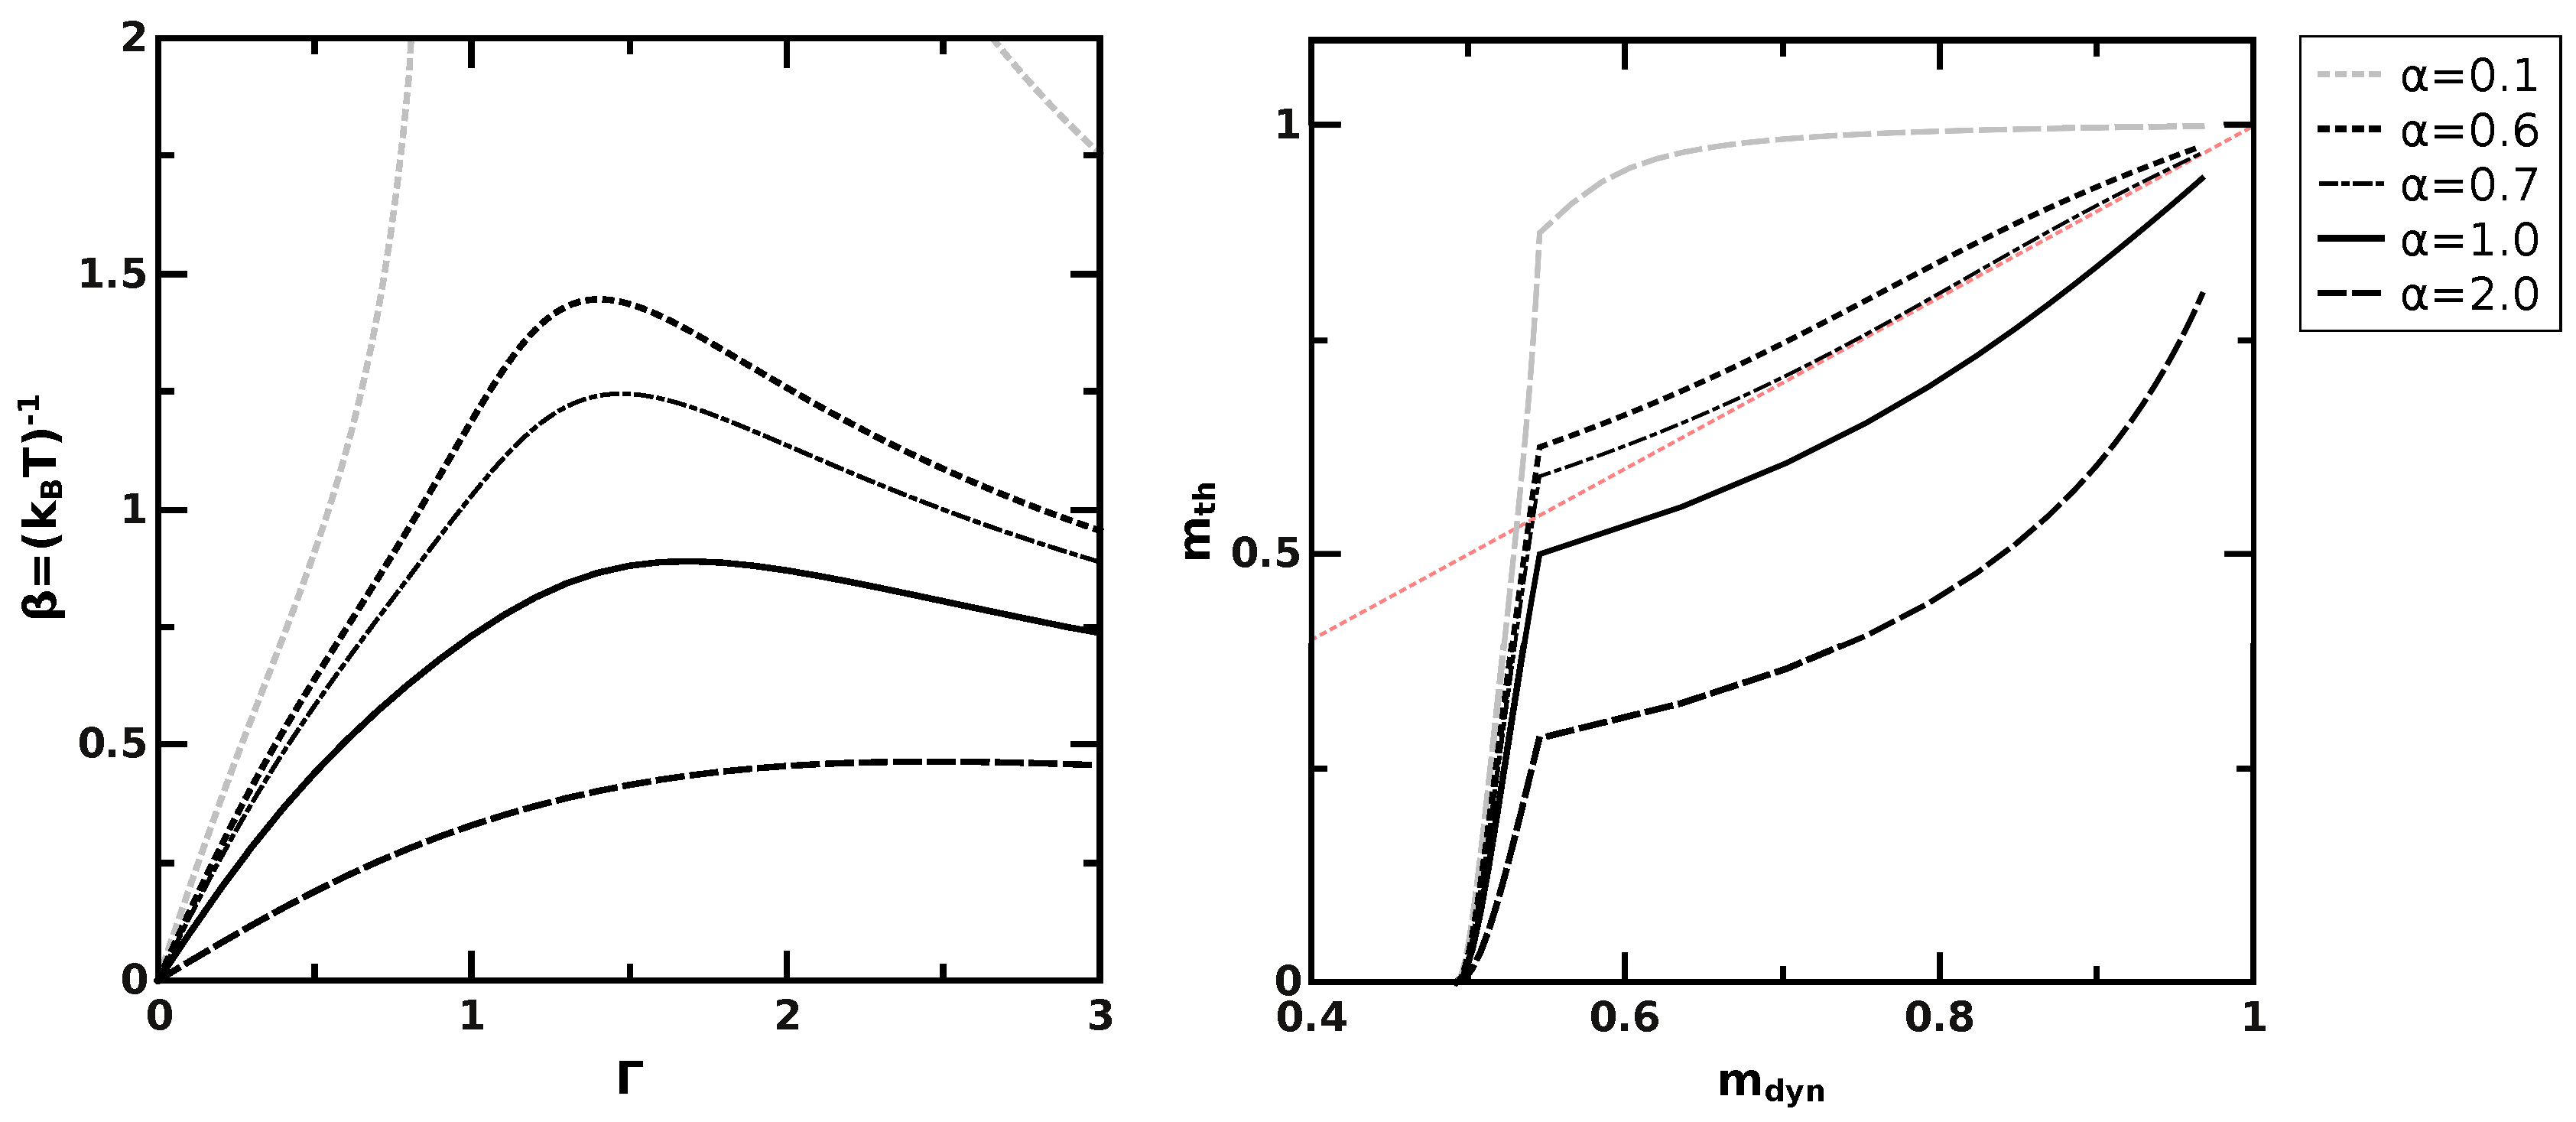
\epsfig{file=quench_vacuum.eps,height=3.0in,width=6.0in}
\caption{Left panel: Plots of the inverse temperature $\beta=(k_BT)^{-1}$ as a function of $\Gamma$ obtained by solving equation~\ref{eq:tempsolve1} for different values of $\alpha$ as shown in the legend. Right panel: Plots of the 'thermal' magnetization $m_{th}$, obtained from eq~\ref{eq:mth}, for a particular value of $\beta$, plotted against the values of the dynamical time-averaged magnetization $m_{dyn}$ obtained from eq~\ref{eq:mdyn1} for the same value of $\beta$. The values of $\beta$ are chosen for a particular value of $\Gamma$ and $\alpha$ from the left panel data. Each curve contains data for a particular value of $\alpha$, and follows the same legend as the left panel. The values of $\Gamma$ for a particular $\alpha$ are the same as the abscissa of the left panel. For each curve, the path of increasing $\Gamma$ starts from the leftmost point and heads rightwards. Note that the QCP is at $\Gamma=1$, and $\lim_{\alpha\rightarrow0}\beta(\Gamma=1)$ diverges. Note that the region $m_{th}=m_{dyn}$ is 
shown in red as a dotten line.}
\label{fig:vacquench}
\end{figure}
The time-averaged dynamical magnetization can be obtained from eq~\ref{eq:mdyn} and~\ref{eq:mop} as
\begin{equation}
\label{eq:mdyn1}
m_{dyn}=\sum _k\frac{(\Gamma -\cos{k})^2}{\left(\Gamma-\cos{k}\right)^2+\alpha ^2 \sin^2{k}}=\frac{1}{2\pi}\int^\pi_{-\pi}\mathrm{d}k\quad \frac{(\Gamma -\cos{k})^2}{\left(\Gamma-\cos{k}\right)^2+\alpha ^2 \sin^2{k}}.
\end{equation}
where we have usind the fact that, for particle vacuum state, $\langle\sigma_y\rangle=0$, and $\langle\sigma_z\rangle=1$. Also, we have taken the continuum 'thermodynamic' limit of large-$N$ in order to arrive at the integral in the equation above.

In order for thermalization to hold, the necessary condition is for $m_{th}$ from eq~\ref{eq:mth} to be equal to $m_{dyn}$. In this particular instance, the equality evaluates to
\begin{equation}
\int^\pi_{-\pi}\mathrm{d}k\quad \left(1-2|v_k|^2\right)\tanh{\beta E_k} = \int^\pi_{-\pi}\mathrm{d}k\quad \frac{(\Gamma -\cos{k})^2}{\left(\Gamma-\cos{k}\right)^2+\alpha ^2 \sin^2{k}},
\end{equation}
where $\beta$ is obtained from eq~\ref{eq:tempsolve1}. The two quantities are plotted in the right panel of fig~\ref{fig:vacquench} for different values of $h,\Gamma$, where the inverse temperatures $\beta$, obtained by solving eqn~\ref{eq:tempsolve} for different values of $h,\Gamma$, are shown in the left panel. The system can only be said to 'thermalize' in any meaningful sense, for points that lie on the line (indicated in red on the right panel) given by $m_{th}=m_{dyn}$. According to the numerics in the figure above, this only appears to be happening around a critical value $\alpha\approx0.7$ for large $\Gamma\geq 1$.

\subsection{Quench in chemical potential $\Gamma$}
Another interesting possibility is a rapid quench in the chemical potential from an initial value $\Gamma_0$ to $\Gamma$, after which the system is allowed to evolve freely in time. Applying such a quench to the Hamiltonian in question should reproduce
the results obtained by Foini, Cugliandolo and Gambassi in $2012$~\cite{leticia}. Foini \textit{et. al.} investigated the dynamics of a transverse Ising system after a rapid quench in the chemical potential, and obtained thermalized behaviour in the immediate neighbourhood of the quantum critical point. Their Hamiltonian matches ours in the thermodynamic limit provided periodic boundary conditions are taken.

\begin{figure}[h!bt]
\ 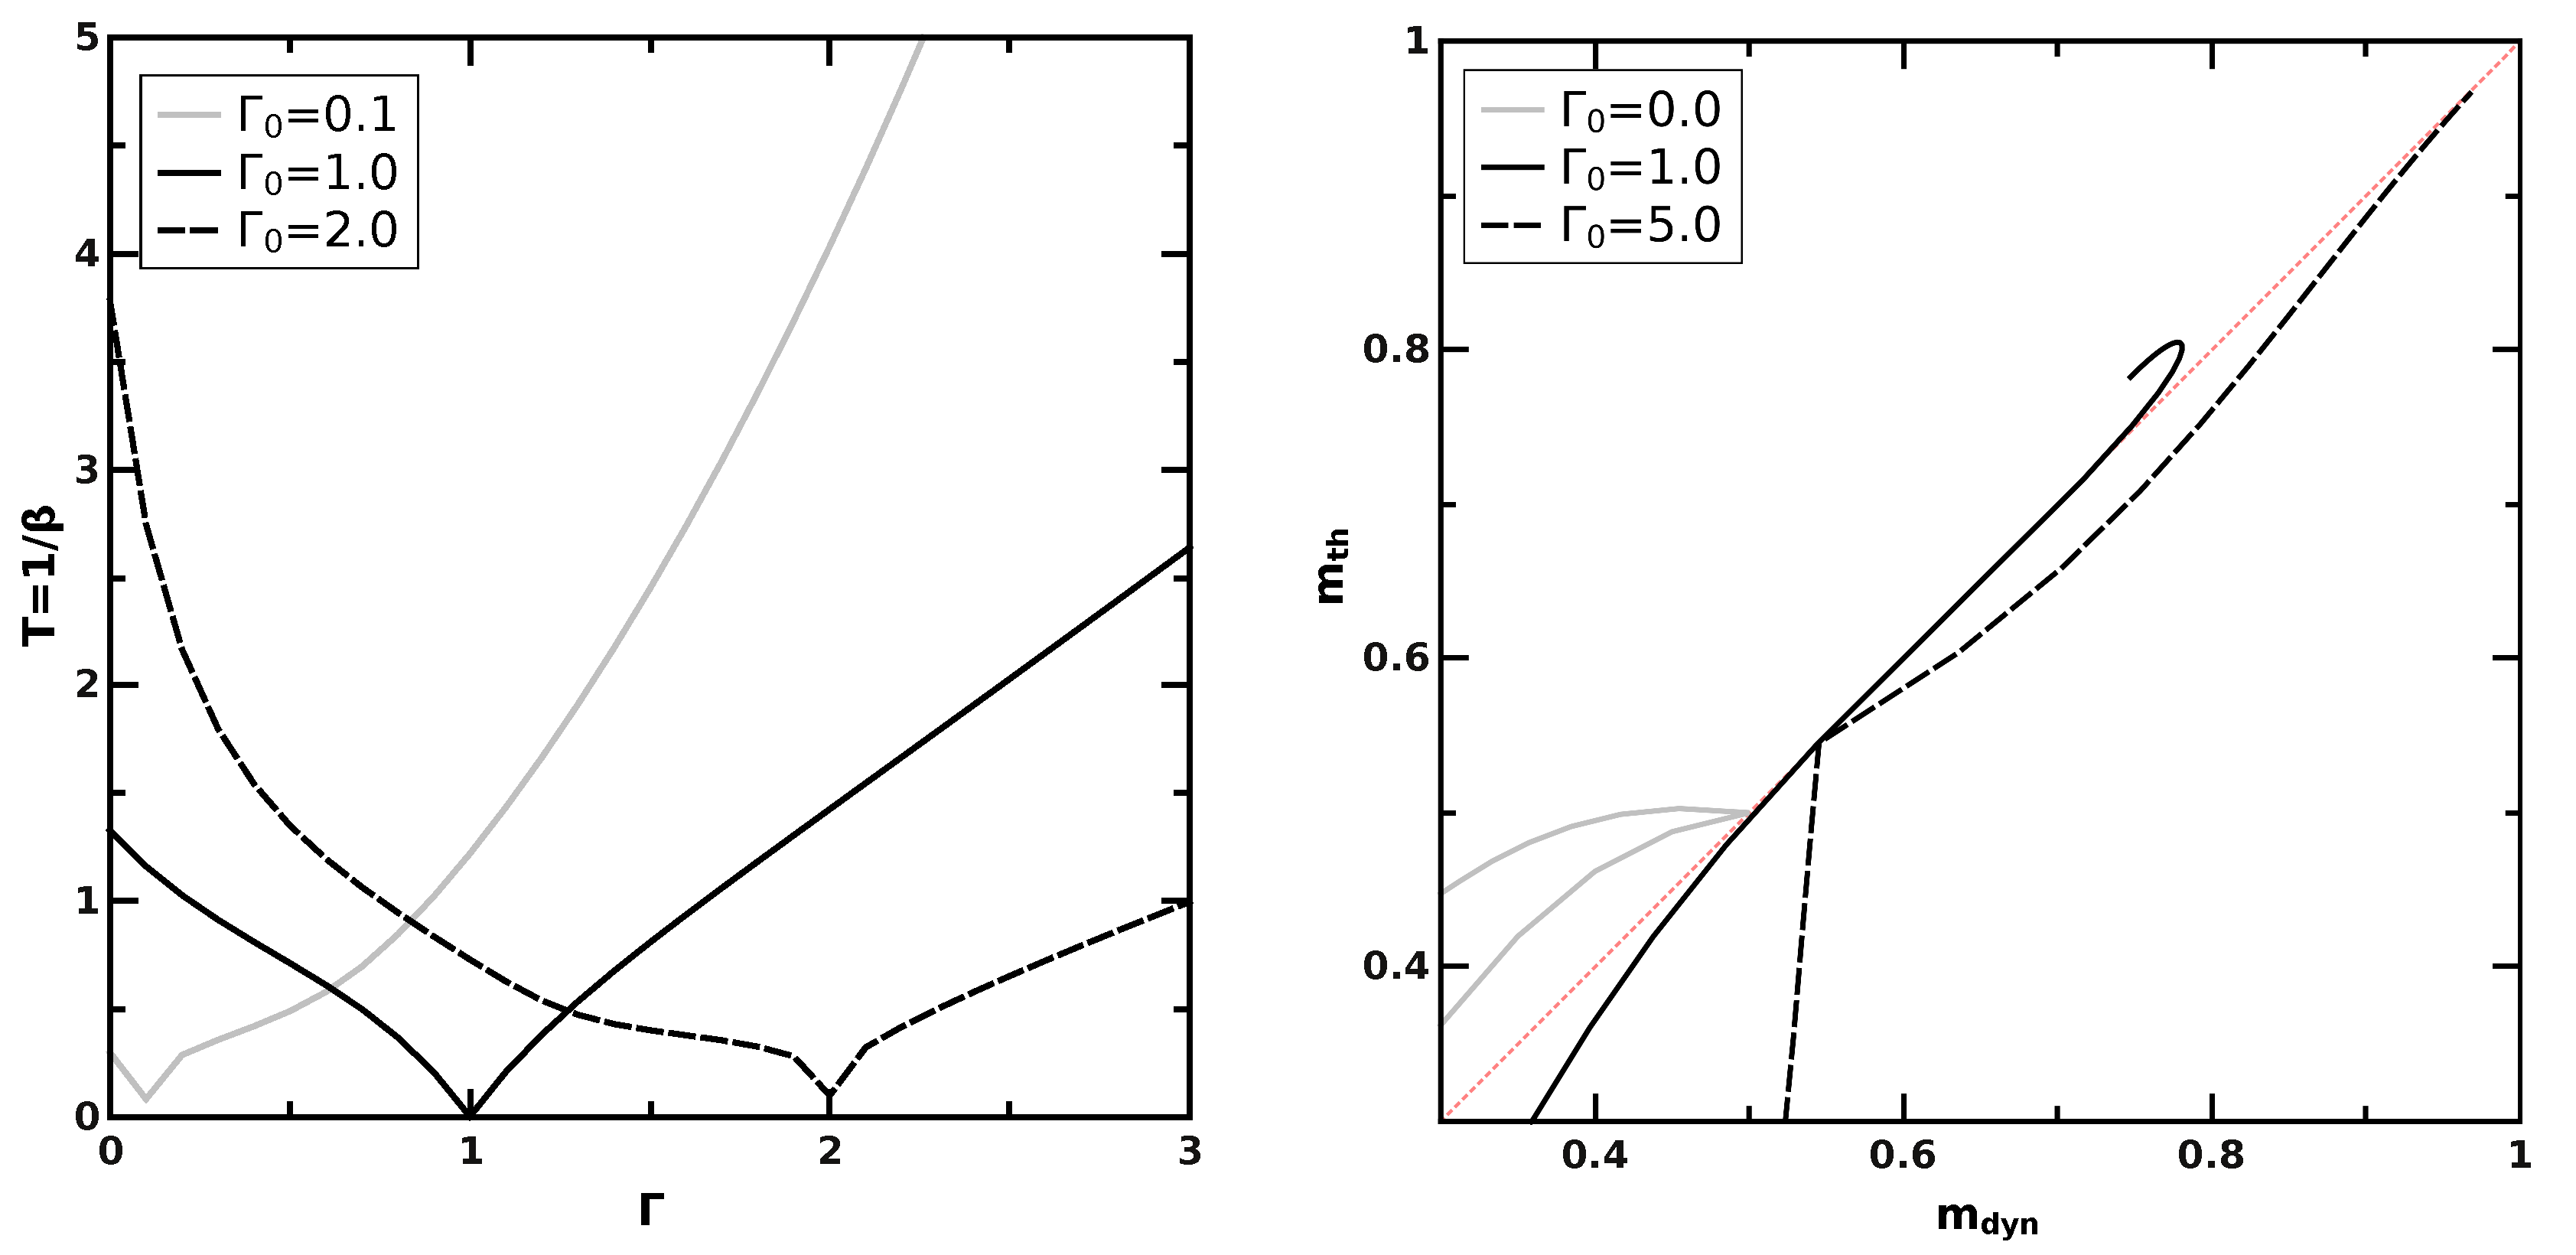
\epsfig{file=quench_gamma.eps,height=3.0in,width=6.0in}
\caption{Left panel: Plots of the temperature $T=(k_B\beta)^{-1}$ as a function of $\Gamma$ obtained by solving equation~\ref{eq:tempsolve2} for different values of $\Gamma_0$ as shown in the legend. Here, $\alpha=1$. Right panel: Plots of the 'thermal' magnetization $m_{th}$, obtained from eq~\ref{eq:mth}, for a particular value of $\beta$, plotted against the values of the dynamical time-averaged magnetization $m_{dyn}$ obtained from eq~\ref{eq:mdyn2} for the same value of $\beta$. The values of $\beta$ are chosen for the values of $\Gamma_0$ in the legend. Each curve contains data for a particular value of $\Gamma_0$. The values of $\Gamma$ for a particular $\Gamma_0$ are the same as the abscissa of the left panel. For each curve, the path of increasing $\Gamma$ starts from the leftmost point and heads rightwards. Note that the QCP is at $\Gamma=1$.Note that the region $m_{th}=m_{dyn}$ is shown in red as a dotten line.}
\label{fig:chempotquench}
\end{figure}

Thus, the initial state $|\Psi_0\rangle$ is
\begin{equation}
\label{eq:psi0}
|\Psi_0\rangle=\prod_k \left(u^0_k-iv^0_kc^\dagger_{k}c^\dagger_{-k}\right)|0\rangle,
\end{equation}
where the coefficients
\begin{eqnarray}
\label{eq:ukvk}
 u^0_k,(v^0_k) &=& \sqrt{\frac{E^0_k+(-) f^0_k}{2E^0_k}},\nonumber \\
 E^0_k &\equiv& \sqrt{\left(f^0_k\right)^2+\Delta^2_k},\nonumber \\
 f^0_k &\equiv& \Gamma_0 -\cos{k},\nonumber \\
 \Delta_k &\equiv& \alpha\sin{k}.
\end{eqnarray}
The 'energy' of the state $|\Psi_0\rangle$, relative to the ground state, is given by
\begin{eqnarray}
E_0 &=& \langle\Psi_0|\mathrm{H}|\Psi_0\rangle \nonumber \\
    &=& -\frac{\mathrm{N}}{2\pi}\int^\pi_{-\pi}\mathrm{d}k\quad\bigg\{2 u^0_k v^0_k \sin{k}-(\Gamma -\cos{k}) \left[1-2 \left(v^0_k\right)^2\right]\bigg\}
\end{eqnarray}
The equivalent temperature of thermalization can be obtained by solving for $\beta$ from the eq~\ref{eq:tempsolve} to yield
\begin{equation}
\label{eq:tempsolve2}
\int^\pi_{-\pi}\mathrm{d}k\quad\bigg\{(\Gamma -\cos{k}) \left[1-2 \left(v^0_k\right)^2\right]-2 u^0_k v^0_k \sin{k}\bigg\} = \int^{\pi}_{0}\mathrm{d}k \quad E_k \tanh{\beta E_k}.
\end{equation}
The time-averaged dynamical magnetization can be obtained from eq~\ref{eq:mdyn} and~\ref{eq:mop} as
\begin{equation}
\label{eq:mdyn2}
m_{dyn}=\frac{1}{2\pi}\int^\pi_{-\pi}\mathrm{d}k\quad  \frac{\left(\Gamma -\cos{k}\right) \left[\left(\Gamma -\cos{k}\right) \left(-\Gamma_0+\cos{k}\right)+|\sin{k}| \sin{k}\right]}{\left(-1-\Gamma ^2+2 \Gamma  \cos{k}\right) \sqrt{1+\Gamma_0^2-2 \Gamma_0 \cos{k}}},
\end{equation}
where we have usind the fact that, for particle vacuum state, $\langle\sigma_y\rangle=2u^0_kv^0_k$, and $\langle\sigma_z\rangle=1-2(v^0_k)^2$. Also, we have taken the continuum 'thermodynamic' limit of large-$N$ in order to arrive at the integral in the equation above.

In order for thermalization to hold, the necessary condition is for $m_{th}$ from eq~\ref{eq:mth} to be equal to $m_{dyn}$ from eqn~\ref{eq:mdyn2}, where $\beta$ for $m_{th}$ is obtained from eq~\ref{eq:tempsolve2}. The two quantities are plotted in the right panel of fig~\ref{fig:chempotquench} for different values of , and the inverse temperatures $\beta$, obtained by solving eqn~\ref{eq:tempsolve2} for different values of  are shown in the left panel. The system can only be said to 'thermalize' in any meaningful sense, for points that lie on the line (indicated in red on the right panel) given by $m_{th}=m_{dyn}$. According to the numerics in the figure above, this appears to occur in the immediate neighborhood of the quantum critical point at $\Gamma=1$ for $\Gamma\gtrsim1$  for all values of $\Gamma_0$. This figure reproduces exactly the results depicted in Fig.3 of Foini \textit{et. al.}~\cite{leticia}, verifying the reliability and authenticity of our numerics.

\subsection{Lattice size quench}
We can choose a different initial condition for the system as well. We now choose the initial condition to be the adiabatic ground state for the Hamiltonian with a smaller number of sites $M<N$. Physically, this would amount to a rapid quench of the system from the ground state of a lattice with $M$ sites to the final lattice. In that case, the initial state is 
\begin{equation}
 |\Psi_0\rangle = \prod_{q\in \mathcal{B}} \left(u_q-iv_qc^\dagger_{q}c^\dagger_{-q}\right)|0\rangle,
\end{equation}
where $\mathcal{B}$ is the Brillouin zone spanned by the $M$ momenta $q$. The momenta are tagged by integer $m$, where $q=-\pi+m (2\pi/M)$. In the full Brillouin zone $\mathcal{W}$, the momenta $k$ can be tagged by integer $n$, where $k=-\pi+n (2\pi/N)$. A momentum from $\mathcal{B}$ will equal that from $\mathcal{W}$ only if there exist integer pairs such that $n/m = N/M$ with $n,m<N,M$ respectively. If we choose $N,M$ to have no common factors, then this never happens, and the momenta in $\mathcal{B}$ are completely disjoint with those from $\mathcal{W}$ (\textit{i.e} $\mathcal{B}\cap\mathcal{W}=\emptyset$). If, however, the two site numbers do have common factors, then there exist momenta (denoted by $s$) in $\mathcal{B}$, which are tagged with integers $m<M$, for which $\ni n<N$ such that $m/n=M/N$, thus making the momenta $s\in\mathcal{B}\cap\mathcal{W}$. Those momenta that do not obey this condition are denoted by $w$. This allows us to break the initial state into a product of two substates, yielding
\begin{eqnarray}
 \label{eq:ic2}
 |\Psi_0\rangle &=& \prod_{s\in{\left(\mathcal{B}\cap\mathcal{W}\right)}} \left(u_s-iv_sc^\dagger_sc^\dagger_{-s}\right)\otimes\prod_{w\in{\left[\mathcal{W}\cup\left(\mathcal{B}\cap\mathcal{W}\right)\right]^c}} \left(u^0_w-iv^0_wc^\dagger_wc^\dagger_{-w}\right) |0\rangle \nonumber \\
 &=& \prod_{s\in{\left(\mathcal{B}\cap\mathcal{W}\right)}} \left(u_s-iv_sc^\dagger_sc^\dagger_{-s}\right)|0\rangle \otimes\prod_{w\in{\left[\mathcal{W}\cup\left(\mathcal{B}\cap\mathcal{W}\right)\right]^c}} |0\rangle
\end{eqnarray}
Note that $\mathcal{B}\cup\mathcal{W}=U$, the universal set, and so if $\mathcal{B}\cap\mathcal{W}=\emptyset$, then the above expression reduces to a single product of momenta $w$ over $\mathcal{W}^c=\mathcal{B}$. Finally, based on eqn~\ref{eq:tempsolve} the effective temperature can be obtained by solving for $\beta$ the equation
\begin{equation}
\langle\Psi_0|\mathrm{H}|\Psi_0\rangle = \sum_{k\in\mathcal{W}}  E_k \tanh{\beta E_k},
\end{equation}
where the continuum limit has not been taken. The lhs of the above can be simplified to yield
\begin{multline}
\langle\Psi_0|\mathrm{H}|\Psi_0\rangle = \prod_{p\in{\left[\mathcal{W}\cup\left(\mathcal{B}\cap\mathcal{W}\right)\right]^c}} \langle\phi_p(0)| \otimes\\
\prod_{q\in{\left(\mathcal{B}\cap\mathcal{W}\right)}} \langle\psi_q(0)|\sum_{k\in\mathcal{W}}\mathrm{H}_k|\prod_{s\in{\left(\mathcal{B}\cap\mathcal{W}\right)}} |\psi_s(0)\rangle
\otimes\\
\prod_{w\in{\left[\mathcal{W}\cup\left(\mathcal{B}\cap\mathcal{W}\right)\right]^c}} |\phi_w(0)\rangle,
\end{multline}
where $|\phi_k(0)\rangle=(u^0_k-iv^0_kc^\dagger_kc^\dagger_{-k})|0\rangle=|0\rangle$, and $|\psi_k(0)\rangle=(u_k-iv_kc^\dagger_kc^\dagger_{-k})|0\rangle\neq|0\rangle$. The above can be simlified further by using the fact that $\langle\psi_p(0)|\psi_w(0)\rangle=\delta_{pw}$, and the fact that
\begin{equation}
\mathrm{H}=\sum_{k\in\mathcal{W}}\mathrm{H}_k=\sum_{k\in\left(\mathcal{B}\cap\mathcal{W}\right)}\mathrm{H}_k + \sum_{q\in\left[\mathcal{B}\cup\left(\mathcal{B}\cap\mathcal{W}\right)\right]^c }\mathrm{H}_q.
\end{equation}
This yields
\begin{eqnarray}
 \langle\Psi_0|\mathrm{H}|\Psi_0\rangle &=& \sum_{k\in\left(\mathcal{B}\cap\mathcal{W}\right)}\langle\psi_k(0)|\mathrm{H}_k|\psi_k(0)\rangle + \sum_{q\in\left[\mathcal{B}\cup\left(\mathcal{B}\cap\mathcal{W}\right)\right]^c}\langle0|\mathrm{H}_k|0\rangle \nonumber \\
                                        &=& \sum_{k\in\left(\mathcal{B}\cap\mathcal{W}\right)}E_k+\sum_{q\in\left[\mathcal{B}\cup\left(\mathcal{B}\cap\mathcal{W}\right)\right]^c}\left(\Gamma-\cos{q}\right).
\end{eqnarray}
Thus, the equation for obtaining $\beta$ simpifies to 
\begin{equation}
\label{eq:tempsolve3}
\sum_{k\in\left(\mathcal{B}\cap\mathcal{W}\right)}E_k + \sum_{q\in\left[\mathcal{B}\cup\left(\mathcal{B}\cap\mathcal{W}\right)\right]^c}\left(\Gamma-\cos{q}\right) = \sum_{s\in\mathcal{W}}  E_s \tanh{\beta E_s}.
\end{equation}
Using arguments similar to those in the previous subsections, the expectation value of the magnetization operator in the Heisenberg representation is
\begin{eqnarray}
{m}(t)   &=&  \langle\Psi_0|e^{-i\sum_{p\in\mathcal{W}}\mathrm{H}_p t}\left[\sum_{k\in\mathcal{W}}\sigma^{(k)}_z\right]e^{i\sum_{p\in\mathcal{W}}\mathrm{H}_p t}|\Psi_0\rangle  \nonumber \\
              &=&  \sum_{k\in\mathcal{W}} \langle\Psi_0|e^{-i\mathrm{H}_k t}\sigma^{(k)}_z e^{i\mathrm{H}_k t}|\Psi_0\rangle \nonumber \\
              &=& \sum_{k\in{\left(\mathcal{B}\cap\mathcal{W}\right)}} \langle\psi_k(0)|e^{-i\mathrm{H}_k t}\sigma^{(k)}_z e^{i\mathrm{H}_k t}|\psi_k(0)\rangle + \sum_{q\in\left[\mathcal{B}\cup\left(\mathcal{B}\cap\mathcal{W}\right)\right]^c } \langle0|e^{-i\mathrm{H}_q t}\sigma^{(q)}_z e^{i\mathrm{H}_q t}|0\rangle
\end{eqnarray}
Now, we can apply eqn~\ref{eq:mop}, average out all oscillatory terms, and apply eqns~\ref{eq:ukvk} and~\ref{eq:icg} to get 
\begin{equation}
\label{eq:mdyn3}
 m_{dyn}= \sum_{k\in{\left(\mathcal{B}\cap\mathcal{W}\right)}} m^{(k)}_{1}  + \sum_{q\in\left[\mathcal{B}\cup\left(\mathcal{B}\cap\mathcal{W}\right)\right]^c } m^{(q)}_{2},
\end{equation}
where the magnetic functions
\begin{eqnarray}
m^{(k)}_{1} &=& \begin{array}{ll}
 \bigg\{ & 
\begin{array}{ll}
 \left(\Gamma-\cos{k}\right) \quad \frac{\left(\Gamma-\cos{k}\right)^2-\alpha^2  \sin^2{k}}{\left[\left(\Gamma-\cos{k}\right)^2+\alpha^2  \sin^2{k}\right]^{3/2}} &\forall k \in [-\pi,0) \\
 \frac{\left(\Gamma-\cos{k}\right)}{\sqrt{\left(\Gamma-\cos{k}\right)^2+\alpha^2  \sin^2{k}}} & \forall k \in [0,\pi]  \\
\end{array}
 \\
\end{array} \nonumber \\
m^{(k)}_{2} &=& \frac{\left(\Gamma-\cos{k}\right)^2}{\left(\Gamma-\cos{k}\right)^2+\alpha^2  \sin^2{k}}.
\end{eqnarray}
In order for thermalization to work, this expression must equal to $m_{th}$ from eqn~\ref{eq:mth} with $\beta$ as the solution to eq~\ref{eq:tempsolve3}. The two are compared in the right panels of fig~\ref{fig:latsizequench} for $M=200$, $N=400$ (top panel), and $M=300$, $N=400$ (bottom panel). The left panels show a plot of temperature $T=(k_B\beta)^{-1}$ obtained by solving eq~\ref{eq:tempsolve3}. For the stronger quench (top panel), we see thermalization at small values of $\alpha$, but significant departure for larger $\alpha$. For the weaker quench, the same trends are qualitatively seen, although thermalization for small $\alpha$ is much weaker than the previous case.

\begin{figure}[h!bt]
\ 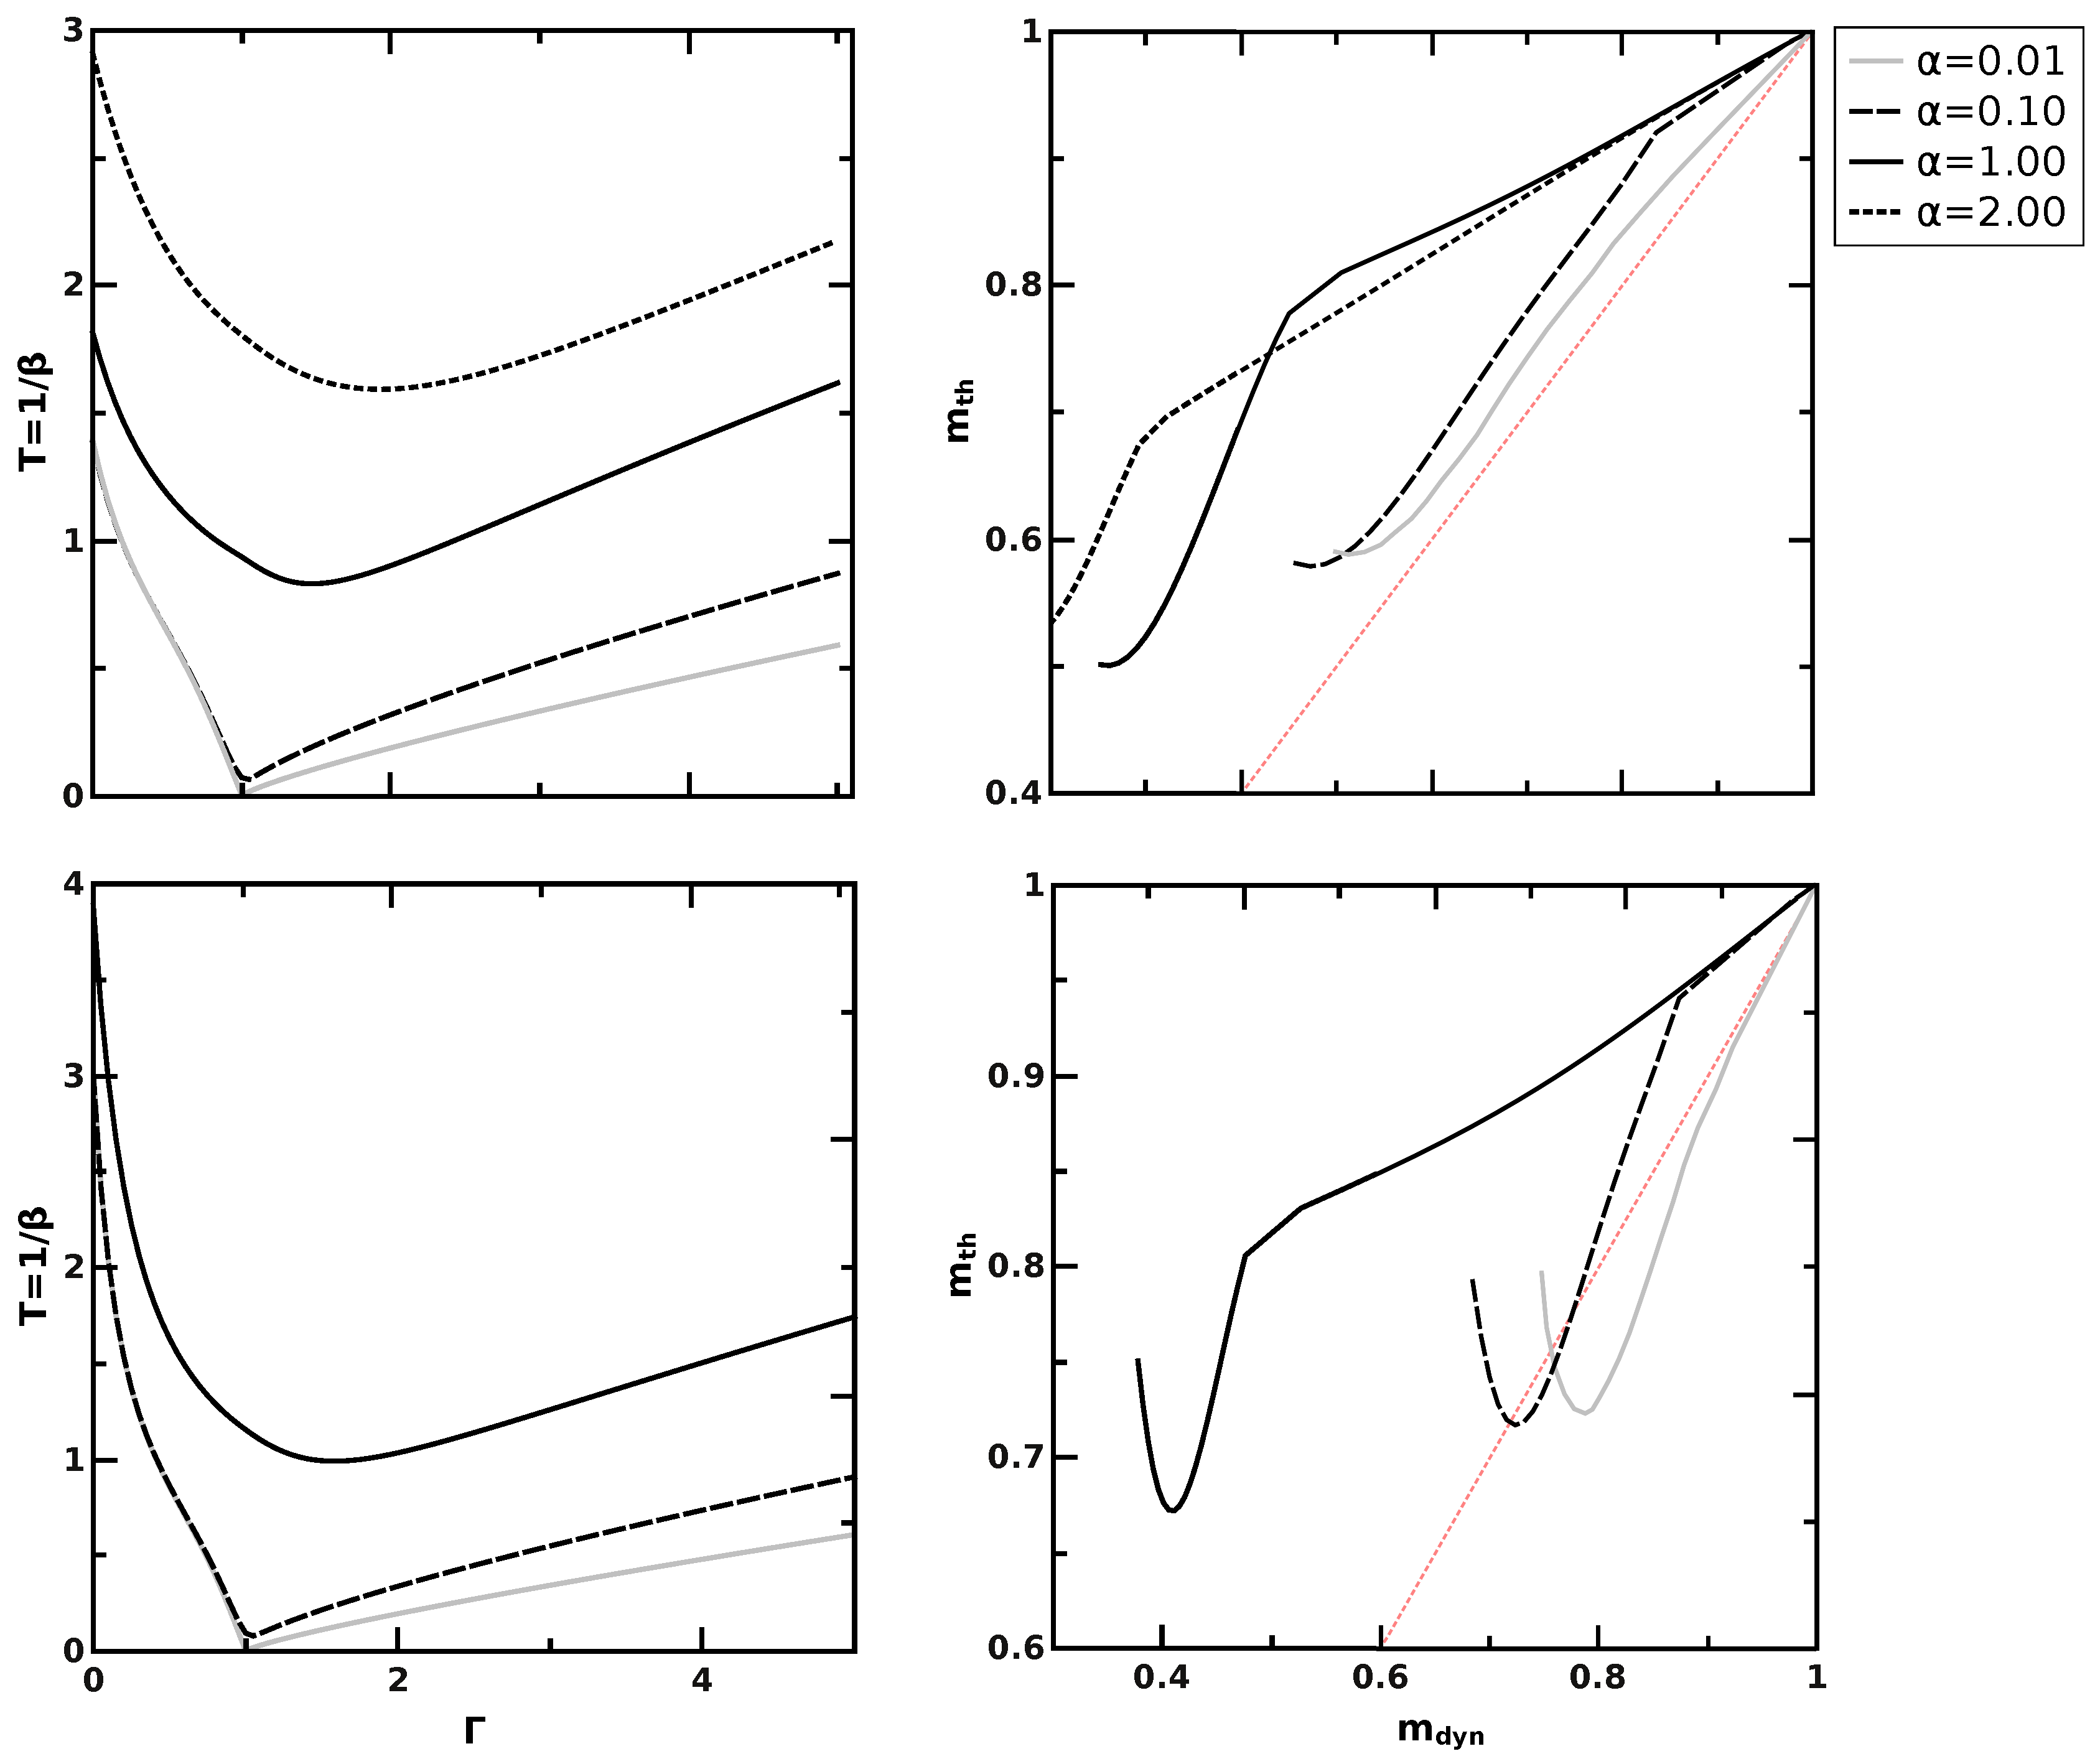
\epsfig{file=latq_N_400_M_200_300.eps,height=6.0in,width=6.5in}
\caption{Left panels: Plots of the temperature $T=(k_B\beta)^{-1}$ as a function of $\Gamma$ obtained by solving equation~\ref{eq:tempsolve3} for different values of $\alpha$ as shown in the legend. Right panels: Plots of the 'thermal' magnetization $m_{th}$, obtained from eq~\ref{eq:mth}, for a particular value of $\beta$, plotted against the values of the dynamical time-averaged magnetization $m_{dyn}$ obtained from eq~\ref{eq:mdyn3} for the same value of $\beta$. The values of $\beta$ are chosen for the values of $\alpha$ in the legend. Each curve contains data for a particular value of $\alpha$. The values of $\Gamma$ for a particular $\alpha$ are the same as the abscissae of the left panels. For each curve, the path of increasing $\Gamma$ starts from the leftmost point and heads rightwards. Note that the QCP is at $\Gamma=1$.Note that the region $m_{th}=m_{dyn}$ is shown in red as a dotten line. The quenches have been performed from a lattice of size $M$ to a final resting size $N>M$. For the top panels,
 $M=200$, $N=400$, and for the bottom panels, $M=300$, $N=400$.}
\label{fig:latsizequench}
\end{figure}


\begin{comment}
 
\section{\sc  Testing the ETH Hypothesis for a driven system}
\label{sec:eth:drv}

\textbf{Warning:Old Notation}\\


Another approach can be to use the RWA dynamics to test the validity of the Eigenstate Thermalization Hypothesis in quantum many body quenching. The base Hamiltonian in eq\ \ref{eq:hamiltonian:su2} can be randomized as shown in section~\ref{sec:tls} and the drive applied either to the amplitude $\lambda$ or the chemical potential $h$. The first subsection below discusses the former case and the next subsection discusses the latter. In both cases, we want the time dependent parameter $p(\tau)$ to exponentially travel from an initial value $p_0$ to a final value $p_1$ while being driven periodically. Thus, a time dependence of the form
\begin{equation}
p(\tau) = p_0 + \left( p_1-p_0\right)\left(1-e^{-{\omega \tau}/{2\pi}}\cos{\Omega \tau}\right)
\end{equation}
is used. We note that, at $\tau=0$, $p(\tau)=p_0$, and at $\tau\rightarrow\infty$, $p(\tau)\rightarrow p_1$. We also note that, although this Hamiltonian is aperiodic in time, we can operate in a regime where $\Omega=N\omega$, $N$ is a positive integer, and $N\gg1$. In this regime, the Gaussian modulation in the amplitude can be roughly taken to be constant in a "time-slice" that is $\mathcal{O}(T)$ long~\cite{
mypapers}. Thus, at a time $t$ after $n$ such "time-slices", when $\tau=nT+t$,
\begin{equation}
\label{eq:lambdat}
 p(\tau)\approx p(n;t)\equiv p_0 + \left(p_1-p_0\right)\left(1-e^{-n}\cos{\Omega t}\right).
\end{equation}
After making this approximation, $H_k(\tau)=H_k(n;t)$ becomes periodic in time during each time slice, and can be solved using standard techniques for periodically driven quantum systems, such as Floquet theory~\cite{mypapers}, the Landau-Zener formula~\cite{landau:lzformula,zener:lzformula,wittig:lzformula} with St\"uckelberg interferometry~\cite{stuckelberg,review:lzstls}, or the Rotating Wave Approximation (RWA)~\cite{arnabdas}. The signal when $p=\lambda$ $p_0=0$, and $p_1=\lambda_0$ is plotted for representative parameters in fig~\ref{fig:quench}.
\begin{figure}[h!bt]
\ 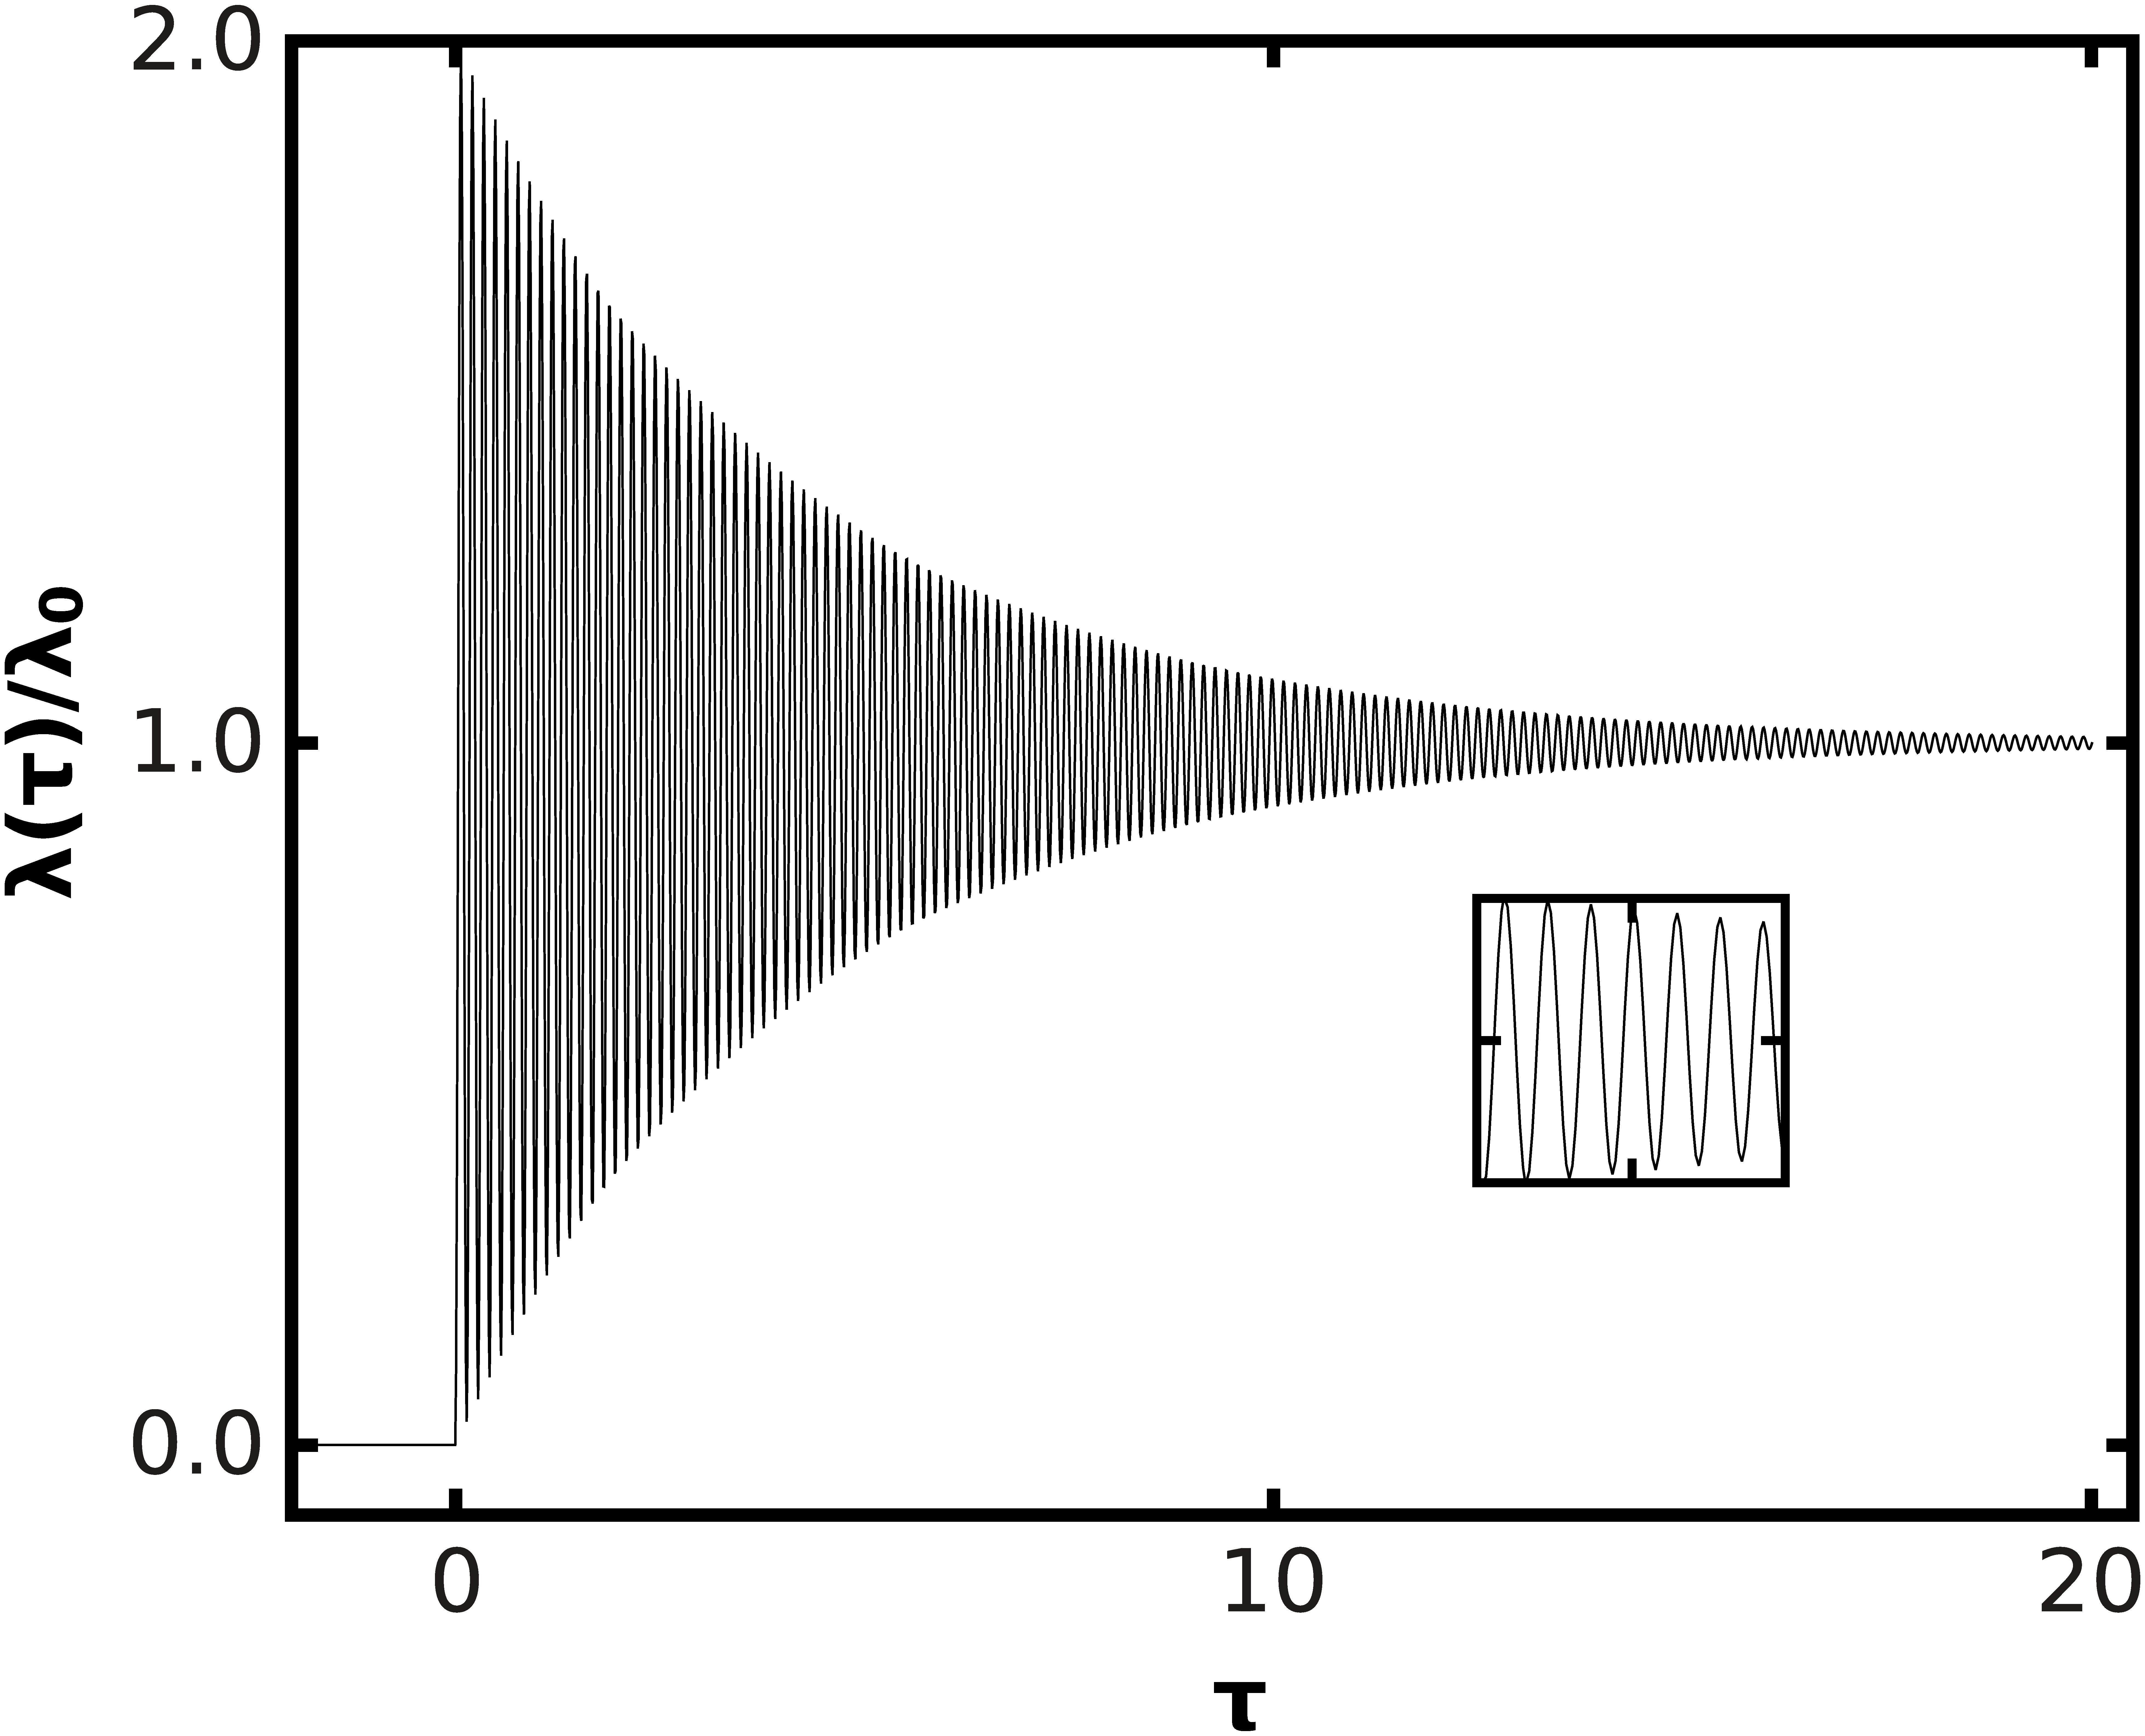
\epsfig{file=quench_signal.eps,height=2.5in,width=3.33in}
\caption{A representative time dependence of $\lambda(\tau)$ from eqns~\ref{eq:hamilt:driven}. The frequency of the amplitude modulation is taken to be $\omega=1.5$, with the harmonic modulation frequency $\Omega=30*\omega$. The inset shows a "time-slice" as defined in the text, strobed around $\tau=15.0$. The amplitude can be seen as roughly constant in this time-slice.}
\label{fig:quench}
\end{figure}
\subsection{\sc Driving the Random Perturbation}
\label{subsec:eth:drv:rnd}
We now apply a time-dependent random matrix perturbation to the Hamiltonian $H$ as follows
\begin{eqnarray}
\label{eq:hamilt:driven}
H_k(\tau; r_k)    &=& \left(h-\cos{k}\right)\sigma_z-\left(\Gamma\sin{k}\right)\sigma_y+\lambda(\tau)r_k\sigma_x,\nonumber \\
\lambda(\tau)&=&\lambda_0\left(1-e^{-{\omega \tau}/{2\pi}}\cos{\Omega \tau}\right).
\end{eqnarray}
Here, as in sec.~\ref{sec:eth:sdn}, $r_k$ is a Gaussian random number. This type of amplitude "quenches" the non-integrable part into the system, taking it from an "integrable" system at $\tau=0$ to a non-integrable one at $\tau\gg T\equiv 2\pi/\omega$. In the limit $\Omega\rightarrow 0$, this becomes a monotonic quenching whereby we expect to get an ETH state in the same sense as described in sec,~\ref{sec:eth:sdn} and as predicted by Deutsch~\cite{deutsch}, as well as well as Yurovsky and Olshanii~\cite{olshanii:ipr}. 
We now proceed for the special case of no source term in the Hamiltonian, \textit{i.e} a gapless Hamiltonian with $\Gamma=0$. At the $n^{th}$ time slice, the time-periodic Hamiltonian is 
\begin{eqnarray}
\label{eq:hamilt:gapless:tslice}
H_k(n;t;r_k)&=&(h-\cos{k})\sigma_z+\lambda_0\left(1-e^{-n}\cos{\Omega t}\right) r_k\sigma_x.\nonumber \\
	&\equiv& H^{(0)}_k - V_k(n;t),  
\end{eqnarray}
where $H^{(0)}_k=(h-\cos{k})\sigma_z+\lambda_0 r_k\sigma_x$, and $V_k(n;t)=[\eta^{(n)}_k\Omega/2]\quad\sigma_x \cos{\Omega t}$ with $\eta^{(n)} _k\equiv(2\lambda_0/\Omega)\quad r_ke^{-n}$. We shall proceed to solve the Schr\"odinger equations~\ref{eq:schroedinger} for the Hamiltonian above using the RWA. This method can be shown to be equivalent to using Floquet Theory in the limit of large $\omega$~\cite{review:lzstls}. Following refs,\ \cite{review:lzstls},\ \cite{oliver} and\ \cite{nori}, we transform to a rotating frame  with the operator $W_k(n;t)\equiv\exp{\left[i\int \mathrm{d}t\quad V_k(n;t)\right]}=\exp{\bigg\{i\left[\eta^{(n)}_k\sigma_x/2\right]\quad\sin{\Omega t}\bigg\}}$. In this frame, the state of the system transforms as $|\psi'_k(n;t)\rangle=W_k(n;t)|\psi_k(n;t)\rangle$. The Schr\"odinger equation in this frame reads $H'_k(n;t)|\psi'_k(n;t)\rangle=i\partial_t|\psi'_k(n;t)\rangle$ $\forall k\in\mathcal{W}$, where
\begin{eqnarray}
\label{eq:hamilt:rot}
H'_k(n;t)&=& W_k(n;t)H_k(n;t)W^\dagger_k(n;t)-iW_k(n;t)\frac{\partial}{\partial t}W^\dagger_k(n;t)\nonumber \\
         &=& W_k(n;t)H^{(0)}_kW^\dagger_k(n;t)\nonumber \\
	 &=& \lambda_0r_k\sigma_x + \left(h-\cos{k}\right)e^{-i\eta^{(n)}_k\cos{\Omega t}}\sigma_p+\textit{h.c} \nonumber \\
         &=&\lambda_0r_k\sigma_x+\sum^{\infty}_{m=-\infty} \left(h-\cos{k}\right)J_m[\eta^{(n)}_k]\quad e^{-im\Omega t}\sigma_p+\textit{h.c}.
\end{eqnarray}
Here, $2\sigma_p\equiv \sigma_z+i\sigma_y$, and we have used the generator for Bessel functions \textit{viz.} 
\begin{equation}
\label{eq:besg}
e^{-ix\sin\tau}=\sum^{\infty}_{m=-\infty}J_m[x]\quad e^{-im\tau}
\end{equation}
to simplify the last line of eq\ \ref{eq:hamilt:rot}. We now make the RWA, assuming that $\Omega \gg h$, the dynamics is expected to relax to a steady state after some time. Therefore, only the least rapid oscillations in the Hamiltonian should contribute to any subsequent dynamics. Thus, we retain only the $m=0$ term in eq\ \ref{eq:hamilt:rot} to obtain the RWA Hamiltonian
\begin{equation}
\label{eq:hamilt:rwa}
H'_k(n;t;r_k)\approx H^{rwa}_k(n;t;r_k)=\begin{bmatrix}
                                 \left(h-\cos{k}\right)J_0[\eta^{(n)}_k] & \lambda_0 r_k \\
				  \lambda_0 r_k	& -\left(h-\cos{k}\right)J_0[\eta^{(n)}_k]
                                \end{bmatrix}.
\end{equation}
Writing 
\begin{equation}
|\psi'_k(t)\rangle = \begin{bmatrix}
                      u_k(t) \\
		      -i v_k(t)
                     \end{bmatrix},
\end{equation}
we drop the primes and get the Schr\"odinger equations for the RWA Hamiltonian
\begin{eqnarray}
\label{eq:rwa:schroedinger}
\dot{u}_k(t;r_k) &=& -i\left(h-\cos{k}\right)J_0[\eta^{(n)}_k] u_k(t;r_k)-\lambda_0r_k v_k(t;r_k),\nonumber \\
\dot{v}_k(t;r_k) &=& \lambda_0 r_k u_k(t;r_k)+i\left(h_0-\cos{k}\right)J_0[\eta^{(n)}_k]v_k(t;r_k).
\end{eqnarray}
Defining the vector
\begin{equation}
\label{eq:unitvec}
{\bm{a}}^{(m)}_k\equiv \lambda_0 r_k\hat{y}+\left(h-\cos{k}\right)J_0[\eta^{(m)}_k]\hat{z},
\end{equation}
and the characteristic frequency $\phi^{(n)}_k\equiv|{\bm{a}}^{(m)}_k|=\sqrt{(h-\cos{k})^2J^2_0[\eta^{(n)}_k]+ \lambda^2_0 r^2_k}$,
eqns\ \ref{eq:rwa:schroedinger} can easily be solved to yield
\begin{eqnarray}
\label{eq:rwa:soln}
|\psi_k(n;t;r_k)\rangle               &   =  & \mathcal{U}^{(n)}_k\left(t;r_k\right)|\psi_k(n-1;T;r_k)\rangle,\nonumber \\
\mathcal{U}^{(n)}_k\left(t;r_k\right) &\equiv& \exp{\bigg\{-i\left[\bm{\sigma}\cdot\hat{\bm{a}}^{(n)}_k\right]\phi^{(n)}_k t\bigg\}},\nonumber \\
				      &   =  & \begin{pmatrix}
                              \cos{\left[\phi^{(n)}_kt\right]}-i(h-\cos{k})J_0[\eta^{(n)}_k]\frac{\sin{\left[\phi^{(n)}_kt\right]}}{\phi^{(n)}_k} & -\lambda_0 r_k \frac{\sin{\left[\phi^{(n)}_kt\right]}}{\phi^{(n)}_k} \\
			      \lambda_0 r_k \frac{\sin{\left[\phi^{(n)}_kt\right]}}{\phi^{(n)}_k} & \cos{\left[\phi^{(n)}_kt\right]}+i(h-\cos{k})J_0[\eta^{(n)}_k]\frac{\sin{\left[\phi^{(n)}_kt\right]}}{\phi^{(n)}_k}
                             \end{pmatrix}.\nonumber \\
\end{eqnarray}
In eqn\ \ref{eq:rwa:soln}, we have approximated the state after $n$ time slices in the model above,$|\psi_k(n-1;T;r_k)\rangle$, with the actual state of the system at that time, $|\psi_k(n;0)\rangle$.
\pagebreak

Thus, we have established that, after a time $\tau=nT+t$, the state of the system is given by
\begin{equation}
\label{eq:soln:rwa:phik}
|\psi_k(\tau;r_k)\rangle = U_k(\tau;r_k)|\psi_k(0)\rangle,
\end{equation}
where
\begin{equation}
\label{eq:rwa:fullsoln}
U_k(\tau;r_k)  =  \mathcal{U}^{(n)}_k(t;r_k)\quad \otimes\prod^{n-1}_{m=0} \mathcal{U}^{(n-m-1)}_k(T;r_k).
\end{equation}
The value of observables like magnetization can be computed from the equations above. For instance, the magnetization at the $n^{th}$ time slice   as a function of time, $q_k(\tau;r_k)$, is 
\begin{equation}
\label{eq:mag:def}
q_k(\tau;r_k)\approx q_k(n;t;r_k)\equiv \langle \psi_k(\tau;r_k)|\sigma_z|\psi_k(\tau;r_k)\rangle= \langle \psi_k(0)|U^\dagger_k(\tau;r_k)\sigma_zU_k(\tau;r_k)| \psi_k(0)\rangle.  
\end{equation}
Using eqns.\ \ref{eq:rwa:soln}\ -- \ref{eq:mag:def}, we get
\begin{equation}
\label{eq:qk}
q_k(n;t;r_k) =  \langle \psi_k(0)|\prod^{n-1}_{p=0} \mathcal{U}^{\dagger(p)}_k(T;r_k)\otimes
               \left[\mathcal{U}^{\dagger(n)}_k(t;r_k)\sigma_z\mathcal{U}^{(n)}_k(t;r_k)\right]\otimes\prod^{n-1}_{m=0} \mathcal{U}^{(n-m-1)}_k(T;r_k)| \psi_k(0)\rangle.
\end{equation}
the time dependent part of $q_k(n;t;r_k)$, enclosed in square brackets in the equation above, can be simplified to yield 
\begin{multline}
\label{eq:ztrans}
U^{\dagger(n)}_k(t;r_k)\sigma_zU^{(n)}_k(t;r_k) =\sigma_z\cos^2{\left[\phi^{(n)}_k t\right]}+\left(\hat{\bm{a}}^{(n)}_k\cdot\hat{y}\right)\sigma_x\sin{\left[2\phi^{(n)}_k t\right]}\\
+\bigg\{2\left( \hat{\bm{a}}^{(n)}_k\cdot\hat{y}\right)\left(\hat{\bm{a}}^{(n)}_k\cdot\hat{z}\right)\sigma_y-\left[\left( \hat{\bm{a}}^{(n)}_k\cdot\hat{y}\right)^2-\left( \hat{\bm{a}}^{(n)}_k\cdot\hat{z}\right)^2\right]\sigma_z\bigg\}\sin^2{\left[\phi^{(n)}_k t\right]}.
\end{multline}
If we now perform a local time average of the quantity in eq.\ \ref{eq:ztrans} over the $n^{th}$ time slice\footnote{In the limit $n\rightarrow\infty$, this would correspond to the time-average after the quench.}, it simplifies to
\begin{eqnarray}
\overline{U^{\dagger(n)}_k(t;r_k)\sigma_zU^{(n)}_k(t;r_k)} &=& \left( \hat{\bm{a}}^{(n)}_k\cdot\hat{z}\right) \sigma_z\left[\left( 
							  \hat{\bm{a}}^{(n)}_k\cdot\hat{z}\right)-i\left( \hat{\bm{a}}^{(n)}_k\cdot\hat{y}\right)\sigma_x\right],\nonumber \\
						   &=& \frac{\left(h-\cos{k}\right)J_0[\eta^{(n)}_k]}{\phi^{(n)}_k}\quad\left(\bm{\sigma}\cdot\hat{\bm a}^{(n)}_k\right),
\end{eqnarray}
where we have used the results from eq\ \ref{eq:unitvec} in the last line. Note that, at resonance, \textit{i.e} at the zeros of $J_0[\eta^{(n)}_k]$, the translation above maps the magnetization to $0$ irrespective of the initial magnetization. Thus the system behaves a little differently from the driven Ising or Kitaev models discussed in the literature~\cite{arnabdas}, where the system freezes at the initial state during resonance. Dynamically, we can see that, at resonance, $\phi^{(n)}_k=\lambda_0r_k$ and $\hat{\bm a}^{(n)}_k=\hat{y}$. Thus, the only dynamics that comes out of the resonance is spin precession, which averages out to $0$. Thus, the local time average of the magnetization is
\begin{equation}
\label{eq:mag:timeavg}
\bar{q}_k(n;r_k)=   \frac{\left(h-\cos{k}\right)J_0[\eta^{(n)}_k]}{\phi^{(n)}_k}\quad \langle \psi_k(0)|\prod^{n-1}_{p=0}  \mathcal{U}^{\dagger(p)}_k(T;r_k) \left(\bm{\sigma}\cdot\hat{\bm a}^{(n)}_k\right)\prod^{n-1}_{m=0} \mathcal{U}^{(n-m-1)}_k(T;r_k)| \psi_k(0)\rangle.
\end{equation}
Using eq\ \ref{eq:rwa:soln} at $t=T$, the leftover operator expression in the equation above can be written in terms of the operator
$\prod^{n-1}_{p=0}\exp{\bigg\{i\left[\bm{\sigma}\cdot\hat{\bm{a}}^{(p)}_k\right]\phi^{(p)}_k T\bigg\}}$. To simplify this, we note the commutation relation $\left[\left(\bm{\sigma}\cdot\hat{\bm a}^{(p)}_k\right)\phi^{(p)}_kT,\left(\bm{\sigma}\cdot\hat{\bm a}^{(p+1)}_k\right)\phi^{(p+1)}_kT\right]_-=2i\bm{\sigma}\cdot\left(\hat{\bm a}^{(p)}_k\times\hat{\bm a}^{(p+1)}_k\right)\phi^{(p)}_k\phi^{(p+1)}_kT^2$. Since $\left(\hat{\bm a}^{(p)}_k\times\hat{\bm a}^{(p+1)}_k\right)$ is small enough to ignore, we can approximate this to be $0$ and use the Zassenhaus formula~\cite{zassenhaus} to write
\begin{eqnarray}
\label{eq:zassenhaus}
\prod^{n-1}_{p=0}\exp{\bigg\{i\left[\bm{\sigma}\cdot\hat{\bm{a}}^{(p)}_k\right]\phi^{(p)}_k T\bigg\}} 
& \approx & \exp{\left[iT\sum_p\phi^{(p)}_k\left(\bm{\sigma}\cdot\hat{\bm a}^{(p)}_k\right)\right]},\nonumber \\
&   =     & \cos{\left[|\bm{b}^{(n)}_k|T\right]}+i\left(\bm{\sigma}\cdot\hat{\bm b}^{(n)}_k\right)\sin{\left[|\bm{b}^{(n)}_k|T\right]},\nonumber \\ \bm{b}^{(n)}_k
&  \equiv &\sum^{n-1}_{p=0}{\bm a}^{(p)}_k.
\end{eqnarray}
Substituting the result above into eq\ \ref{eq:mag:timeavg} yields
\begin{multline}
\bar{q}_k(n;r_k)\approx \frac{\left(h-\cos{k}\right)J_0[\eta^{(n)}_k]}{\phi^{(n)}_k}\quad\langle \psi_k(0)\big| \bigg\{\cos{\left(|\bm{b}^{(n)}_k|T\right)}+i\left(\bm{\sigma}\cdot\hat{\bm b}^{(n)}_k\right)\sin{\left(|\bm{b}^{(n)}_k|T\right)}\bigg\}\otimes
\left(\bm{\sigma}\cdot\hat{a}^{(n)}_k\right)\otimes\\
\bigg\{\cos{\left(|\bm{b}^{(n)}_k|T\right)}-i\left(\bm{\sigma}\cdot\hat{\bm b}^{(n)}_k\right)\sin{\left(|\bm{b}^{(n)}_k|T\right)}\bigg\}\big|\psi_k(0)\rangle,
\end{multline}
where $T=2N\pi/\Omega$. Expanding the above expression yields
\begin{multline}
\label{eq:mag:timeavg1}
\bar{q}_k(n;r_k)\approx \frac{\left(h-\cos{k}\right)J_0[\eta^{(n)}_k]}{\phi^{(n)}_k}\quad\bigg\{
\left\langle \bm{\sigma}\cdot\hat{\bm a}^{(n)}_k\right\rangle \cos{\left(2|\bm{b}^{(n)}_k|T\right)}
+\left\langle \bm{\sigma}\cdot\hat{\bm a}^{(n)}_k\times\hat{\bm b}^{(n)}_k\right\rangle \sin{\left(2|\bm{b}^{(n)}_k|T\right)}+\\
2 \left\langle \bm{\sigma}\cdot\hat{\bm a}^{(n)}_k\right\rangle \left(\hat{\bm a}^{(n)}_k\cdot\hat{\bm b}^{(n)}_k\right) \sin^2{\left(|\bm{b}^{(n)}_k|T\right)}
\bigg\}.
\end{multline}
Here, $\left\langle\dots\right\rangle$ denotes the expectation value with respect to $|\psi_k(0)\rangle$. Also, to reiterate previous definitions,
\begin{eqnarray}
\label{eq:reiteration}
\bm{\sigma}	     &\equiv& \sigma_x \hat{x} + \sigma_y \hat{y} + \sigma_z \hat{z},\nonumber \\
\bm{b}^{(n)}_k       &\equiv& \sum^{n-1}_{p=0}\phi^{(p)}_k\hat{\bm a}^{(p)}_k,\nonumber \\
\hat{\bm{a}}^{(p)}_k &\equiv& \frac{1}{\phi^{(p)}_k}\bigg\{\lambda_0 r_k\hat{y}+\left(h-\cos{k}\right)J_0[\eta^{(p)}_k]\hat{z}\bigg\},\nonumber \\
\phi^{(p)}_k	     &\equiv& \sqrt{(h-\cos{k})^2J^2_0[\eta^{(p)}_k]+ \lambda^2_0 r^2_k},\nonumber \\
\eta^{(p)}_k	     &\equiv& \frac{2\lambda_0}{\Omega}\quad r_k e^{-p},
\end{eqnarray}
$J_0[x]$ is the lowest order Bessel function, and $p\in\mathbb{Z}_{\geq 0}$. Also, the initial state
\begin{equation}
|\psi_k(0)\rangle = \begin{pmatrix}
                      +u_k\\
                      -iv_k
                      \end{pmatrix},
\end{equation}
where $u_k(v_k)$ are taken from eqs\ \ref{eq:ukvk} with $\Gamma=0$ (gapless), yielding eq\ \ref{eq:gapless:ic}. Now, we note that, as $n\rightarrow\infty$, $\eta^{(n)}_k\rightarrow 0$, and $J^2_0[\eta^{(n)}_k]\rightarrow 1$. This, in turn, means that $\phi^{(n)}_k\rightarrow e_k\equiv\sqrt{(h-\cos{k})^2+\lambda^2_0r^2_k}$, and $\hat{\bm{a}}^{(n)}_k \rightarrow \left[\lambda_0 r_k\hat{y}+\left(h-\cos{k}\right)\hat{z}\right]/{e_k}$, and finally, 
$\hat{\bm b}^{(n)}_k\rightarrow \hat{y}$, and $|\bm{b}^{(n)}_k|\rightarrow n\lambda_0 r_k$.\footnote{As $n\rightarrow\infty$, $\bm{b}^{(n)}_k\rightarrow \sum^\infty_{p=0}\bigg\{\lambda_0 r_k\hat{y}+\left(h-\cos{k}\right)J_0[\eta^{(p)}_k]\hat{z}\bigg\}\sim n\lambda_0 r_k\hat{y}$, provided $n\gg h$. This happens because $J_0[\eta^{(p)}_k]\leq 1$ $\forall p$, and diverges slowly compared to $\lambda_0 r_k$, which is independent of $p$.} 
Therefore, the local time-averaged magnetization after a quench can be computed from~\ref{eq:mag:timeavg1} to yield
\begin{multline}
\label{eq:mag:timeavg2}
\bar{q}_k(n;r_k)\approx \frac{\left(h-\cos{k}\right)\left[\lambda_0r_ky_k+\left(h-\cos{k}\right)z_k\right]}{(h-\cos{k})^2+ \lambda^2_0r^2_k}\quad\bigg\{ 
\left[1-\frac{\lambda_0r_k}{\sqrt{(h-\cos{k})^2+ \lambda^2_0r^2_k}}\right]\cos{\left(2n\lambda_0 r_kT\right)}+\\
\frac{\lambda_0r_k}{\sqrt{(h-\cos{k})^2+ \lambda^2_0r^2_k}}\bigg\},
\end{multline}
where we have eliminated the $\langle\sigma_x\rangle$ - term, since $\langle\sigma_x\rangle=0$, and have defined $y_k,x_k$ using the initial conditions in eq\ \ref{eq:gapless:ic}, 
\begin{eqnarray}
\label{eq:ykzk}
y_k &\equiv& \left\langle\sigma_y\right\rangle = -2u_kv_k,\nonumber \\
z_k &\equiv& \left\langle\sigma_z\right\rangle = 1-2|v_k|^2.
\end{eqnarray}
We now perform the average over disorder configurations, which amounts to a random average over $r_k$ (henceforth denoted by the operation $\langle \dots \rangle_{\rm rand}$), yielding
\begin{equation}
Q_k\equiv\left\langle\bar{q}_k(n;r_k)\right\rangle_{\rm rand}.
\end{equation}
In order to evaluate the random averages in the equation above, we use the result, $\langle r_k\rangle_{\rm rand}=0$, define the distribution variance $\chi^2\equiv\langle r^2_k \rangle_{\rm rand}$, and use the following result,
\begin{equation}
\label{eq:taylorxpand}
\left\langle\bar{q}_k(n;r_k)\right\rangle_{\rm rand}\approx \bar{q}_k\left(n;\left\langle r_k\right\rangle_{\rm rand}\right)+
\frac{\chi^2}{2} \frac{\partial^2}{\partial^2 r_k}\bar{q}_k(n;r_k)\bigg|_{r_k=0},
\end{equation}
in a manner similar to eq~\ref{eq:taylorxpand:orig} in subsection\ \ref{subsec:imp:rnd}. Applying these results to eq\ \ref{eq:mag:timeavg2} yields an expression for the time-disorder averaged magnetization analogous to eq\ \ref{eq:trandmag} in subsection~\ref{subsec:eth:drv:rnd}
\begin{equation}
\label{eq:mag:timerandavg1}
 Q_k\equiv\left\langle \bar{q}_k(r_k)\right\rangle_{\rm rand} = \left(1-2|v_k|^2\right)\mathcal{D}_k,
\end{equation}
where the distributions
\begin{eqnarray}
\label{eq:rwa:distribs}
\mathcal{D}_k &\equiv& 1 - \left(2n\lambda_0\chi T\right)^2 +  \lambda^2_0 \chi^2\mathcal{T}_k,\nonumber \\
\mathcal{T}_k &\approx& -\frac{1}{(h-\cos{k})^2}.
\end{eqnarray}
This expression has a singularity whenever $h\leq 1$. Whenever $h>1$, the total quantum magnetism, $Q\equiv \sum_k Q_k$ , seems to have two components
\begin{equation}
\label{eq:qthm}
Q = \left[1-\left(2n\lambda_0\chi T\right)^2\right] Q^{\rm qnt}  + \lambda^2_0 \chi^2Q^{\rm thm},
\end{equation}
where $Q^{\rm qnt}=\sum_k 1-2|v_k|^2$ is the initial purely quantum magnetization, and $Q^{\rm thm}=\sum_k \left(1-2|v_k|^2\right)\mathcal{T}_k$ weighs down the microscopic quantum magnetization, $\left(1-2|v_k|^2\right)$, with the 'thermal' distribution $\mathcal{T}_k$. In the limit $\chi,\lambda_0\rightarrow 0$, $Q^{\rm qnt}$ becomes the dominant contributor to the magnetization, whereas $Q^{\rm thm}$ starts to contribute as $\chi$ or $\lambda_0$ is increased. Note, however, that the contribution of $Q^{\rm qnt}$ can be decreased by increasing $\Omega$ without changing the disorder, in marked contrast to the results in subsection\ \ref{subsec:imp:rnd}. Also, in marked contrast to the results in subsection\ \ref{subsec:imp:rnd}, there exists a resonant frequency (for each time slice) $\Omega\approx 4\pi n \lambda_0\chi$, at which the contribution of ${Q}^{\rm qnt}$ disappears, leaving only the contribution of ${Q}^{\rm thm}$. \textbf{Thus, if we can demonstrate that ${\bf Q}^{\rm{\bf thm}}$ is indeed a '
thermal' 
distribution, then 
there exists at least one resonant frequency where the system is purely thermal, with no participation of the quantum magnetism}. Moving on, we note that $Q^{\rm thm}$ is the contribution of the disorder to the magnetization, although large values of $\chi$ will produce higher order contributions from eq\ \ref{eq:taylorxpand}. Near $h\gtrsim 1$, $\mathcal{T}_k$ tends to a delta function that preferentially selects momenta in a small interval about $k=0$ from $\mathcal{W}$. Note that, when we switch from dimensionless units to natural units, $k$ maps to $ka$, and $h$ maps to $2ma^2\epsilon/\hbar^2$, where $m$ is the mass, $a$ the lattice cell size, and $\epsilon$ is the lattice hopping energy.

Now, we attempt to determine whether the contribution of the disorder amounts to any kind of 'thermalization' via the Eigenstate Thermalization Hypothesis (ETH).  To that end, we first note that the 'eigenstates' for each momentum are given by eq\ \ref{eq:unpert:esystem} in the absence of any quenches with the gap $\Gamma=0$. Thus, a purely ensemble average over the eigenstates of the magnetization is 
\begin{equation}
\label{eq:gge}
Q^{\rm gge} = \sum_{k} \left(1-2|v_k|^2\right)\quad \tanh{\left[\beta_k\left(h-\cos{k}\right)\right]}.
\end{equation}
This follows from the partition function $\mathcal{Z}=\prod_k \mathcal{Z}_k$, where $\mathcal{Z}_k=\sum_{\pm}\exp{\left[\pm\beta_k\left(h-\cos{k}\right)\right]}$, and the sum is carried out over the energy eigenvalues of the states in eq \ \ref{eq:unpert:esystem}. The mode-dependent term $\beta_k$, is obtained from the generalized Gibbs ensemble (GGE)\ \cite{rigol:nature, krishnenduda:ethreview}, and corresponds to an integral of the dynamics for each momentum. This quantity can be called a mode dependent 'inverse temperature' once thermalization is justified. Equating $Q^{\rm gge}$ to $Q^{\rm thm}$ necessitates that $\mathcal{T}_k=\tanh{\left[\beta_k\left(h-\cos{k}\right)\right]}$\footnote{If the relation $Q^{\rm gge}-Q^{\rm thm}$ is to hold independently of the underlying lattice structure, then each term in the momentum sum must identically vanish.}, or
\begin{equation}
\label{eq:invtemp}
\beta_k = \frac{-1}{\left(h-\cos{k}\right)}\quad \tanh^{-1}{\left[\frac{1}{\left(h-\cos{k}\right)^2}\right]}\approx-\frac{1}{h^3},
\end{equation}
where the last approximation holds if $h\gg1$\ \footnote{Here, we have used the series $\tanh^{-1}{x}=\sum^\infty_{n=0}\frac{x^{2n+1}}{2n+1}$.}. Using this abovementioned value of $\beta_k$ guarantees thermalization of $Q$ by construction for large $h$. However, as $h$ approaches unity, the temperature becomes 'mode dependent', whose thermodynamic significance is unclear. If $h<1$, singularities in the random averaged distribution destroy thermalization. The two quantities $Q^{\rm thm}$ and $Q^{\rm gge}$ are compared as functions of $h$ in fig\ \ref{fig:thgge:imp}. Here, the thermodynamic limit $\sum_k\rightarrow\frac{1}{2\pi}\int_\mathcal{W}\mathrm{d}k$ has been taken, and the integrations performed numerically using quadratures.

This construct, while necessary for thermalization, may be insufficient. We wish to determine if, long after the quench dies out, the macroscopic observable appears ergodic for our choice of initial conditions. To do so, $\beta_k$ must be convincingly demonstrated to be a 'constant of motion' over the fluctuations of the observables as well. However, the literature in this area does not address the issue of fluctuations. If, however, we require that, for each $k$, the mean square difference between the long-time average of the 'thermal' part of the dynamical magnetization and the ensemble fluctuations in magnetization obtained from the GGE given by $\mathcal{Z}_k$ approaches $0$ in the thermodynamic limit\ \cite{krishnenduda:ethreview,reimann}, we get a discrepancy. To see this, we evaluate the dynamical quantity $q^2_k(n;t;r_k)$ by squaring eqn\ \ref{eq:qk}, insert eq\ \ref{eq:ztrans}, and apply the simplification in eq\ \ref{eq:zassenhaus}. This yields
\begin{equation}
q^2_k(n;t;r_k) \approx \left[{\bm d}^{(n)}_k\left(t\right)\cdot {\bm s}^{(n)}_k \right]^2,
\end{equation}
where
\begin{multline}
\bm{s}^{(n)}_k\equiv
\langle \psi_k(0)| \bigg\{\cos{\left[|\bm{b}^{(n)}_k|T\right]}+i\left(\bm{\sigma}\cdot\hat{\bm b}^{(n)}_k\right)\sin{\left[|\bm{b}^{(n)}_k|T\right]}\bigg\}{\bm \sigma}\\
\bigg\{\cos{\left[|\bm{b}^{(n)}_k|T\right]}-i\left(\bm{\sigma}\cdot\hat{\bm b}^{(n)}_k\right)\sin{\left[|\bm{b}^{(n)}_k|T\right]}\bigg\}|\psi_k(0)\rangle,
\end{multline}
and
\begin{multline}
\label{eq:dvec}
\bm{d}^{(n)}_k\left(t\right) \equiv \left(\hat{\bm{a}}^{(n)}_k\cdot\hat{y}\right)\sin\left[2\phi^{(n)}_k t\right] \hat{x}+ 
2 \left(\hat{\bm{a}}^{(n)}_k\cdot\hat{y}\right) \left(\hat{\bm{a}}^{(n)}_k\cdot\hat{z}\right)\sin^2\left[\phi^{(n)}_k t\right]\hat{y}+\\
\bigg\{\cos^2\left[\phi^{(n)}_k t\right]-\left[\left(\hat{\bm{a}}^{(n)}_k\cdot\hat{y}\right)^2-\left(\hat{\bm{a}}^{(n)}_k\cdot\hat{z}\right)^2\right]\sin^2\left[\phi^{(n)}_k t\right]\bigg\}\hat{z}.
\end{multline}
Thus, the local time average in the $n^{th}$ time slice, $\overline{q^2_k}(n;t;r_k) \approx \overline{(d_x s_x + d_y s_y + d_z s_z)^2}=\overline{d^2_x}s^2_x+\overline{d^2_y}s^2_y+\overline{d^2_z}s^2_z + 2\overline{d_xd_y}s_xs_y + 2\overline{d_yd_z}s_ys_z + 2\overline{d_xd_z}s_xs_z$, where the superscript $(n)$ and subscript $k$ have been removed for clarity. Looking at eq\ \ref{eq:dvec}, we can see that
\begin{eqnarray}
\overline{d^2_x} &=& \frac{1}{2} \left(\hat{\bm{a}}^{(n)}_k\cdot\hat{y}\right)^2,\nonumber \\
\overline{d^2_y} &=& \frac{3}{4}  \left(\hat{\bm{a}}^{(n)}_k\cdot\hat{y}\right) \left(\hat{\bm{a}}^{(n)}_k\cdot\hat{z}\right),\nonumber \\
\overline{d^2_z} &=& \frac{3}{8}\left[\left(\hat{\bm{a}}^{(n)}_k\cdot\hat{x}\right)^2+2\left(\hat{\bm{a}}^{(n)}_k\cdot\hat{z}\right)^2\right]^2 ,\nonumber \\
\overline{d_yd_z} &=& \frac{1}{4}\left(\hat{\bm{a}}^{(n)}_k\cdot\hat{y}\right)\left(\hat{\bm{a}}^{(n)}_k\cdot\hat{z}\right)  
\left[\left(\hat{\bm{a}}^{(n)}_k\cdot\hat{z}\right)^2-2\left(\hat{\bm{a}}^{(n)}_k\cdot\hat{y}\right)^2+4\left(\hat{\bm{a}}^{(n)}_k\cdot\hat{x}\right)^2\right],\nonumber \\
\overline{d_xd_y} &=& \overline{d_xd_z}=0.
\end{eqnarray}
If we now take the limit of large $n$, $\bm{a}^{(n)}_k\rightarrow \lambda_0 r_k \hat{y}+\left(h-\cos{k}\right)\hat{z}$, and $\bm{b}^{(n)}_k\rightarrow n\lambda_o r_k \hat{y}$. Thus
\begin{eqnarray}
\label{eq:davgs}
\overline{d^2_x} &\approx& \frac{1}{2}\quad \frac{\lambda^2_0r^2_k}{\lambda^2_0  r^2_k+\left(h-\cos{k}\right)^2} ,\nonumber \\
\overline{d^2_y} &\approx& \frac{3}{4}\quad \frac{\lambda_0 r_k\left(h-\cos{k}\right)}{\lambda^2_0  r^2_k+\left(h-\cos{k}\right)^2},\nonumber \\
\overline{d^2_z} &\approx& \frac{3}{4}\quad \frac{\left(h-\cos{k}\right)^4}{\left[\lambda^2_0  r^2_k+\left(h-\cos{k}\right)^2\right]^2},\nonumber \\
\overline{d_yd_z} &\approx& \frac{1}{4}\quad{\lambda_0 r_k}\left(h-\cos{k}\right)\quad 
 \frac{\left[\left(h-\cos{k}\right)^2-2\lambda^2_0r^2_k\right]}{\left[\lambda^2_0  r^2_k+\left(h-\cos{k}\right)^2\right]^2},\nonumber \\
\overline{d_xd_y} &=& \overline{d_xd_z}=0.
\end{eqnarray}
In addition, for large $n$,
\begin{eqnarray}
\bm{s}^{(n)}_k &\approx& \langle \psi_k(0)| \bigg[\cos{\left(n\lambda_0r_kT\right)}+i\sigma_y\sin{\left(n\lambda_0r_kT\right)}\bigg]{\bm \sigma}
			  \bigg[\cos{\left(n\lambda_0r_kT\right)}-i\sigma_y\sin{\left(n\lambda_0r_kT\right)}\bigg]|\psi_k(0)\rangle, \nonumber\\
	       &   =   & \left\langle\bm{\sigma}\right\rangle\cos^2{\left(n\lambda_0r_kT\right)}-\frac{i}{2}\left\langle \left[\bm{\sigma},\sigma_y\right]_- \right\rangle\sin{\left(2n\lambda_0r_kT\right)}+\left\langle \sigma_y \bm{\sigma}\sigma_y\right\rangle \sin^2{\left(n\lambda_0r_kT\right)}.
\end{eqnarray}
where $\left\langle\dots\right\rangle$ denotes the expectation value wrt $|\psi_k(0)\rangle$. Thus, $s_x \approx z_k \sin{\left(2n\lambda_0r_kT\right)}$, $s_y \approx y_k$, and  $s_z \approx z_k \cos{\left(2n\lambda_0r_kT\right)}$,
where we have used definitions from eq\ \ref{eq:ykzk}. Plugging these results, together with those of eq\ \ref{eq:davgs}, into  the expression for $\overline{q^2_k}(n;r_k)$ yields
\begin{multline}
\label{eq:magfluct}
\overline{q^2_k}(n;r_k)=
\frac{1}{4 \left[\lambda^2_0r^2_k+(h-\cos{k})^2\right]^2}\quad
 \bigg\{3 \lambda_0 r_k y^2_k  \left[\lambda^2_0 r^2_k+(h-\cos{k})^2\right] (h-\cos{k})+ 2\lambda_0 r_k y_k z_k \\ \left[-2\lambda^2_0 r^2_k+(h-\cos{k})^2\right] (h-\cos{k}) \cos{\left(2n\lambda_0r_kT\right)}+\\
 3 z^2_k (h-\cos{k})^4 \cos^2{\left(2n\lambda_0r_kT\right)}+\\
2 \lambda^2_0 r^2_k z^2_k \left[\lambda^2_0 r^2_k+(h-\cos{k})^2\right]
\sin^2{\left(2n\lambda_0r_kT\right)}\bigg\}.
\end{multline}
Note from the above that the second order partial derivative
\begin{equation}
\label{eq:partial2}
\frac{\partial^2}{\partial^2 r_k} \overline{q^2_k}(n;r_k)\bigg|_{r_k=0}=-\left(1-2|v_k|^2\right)^2\quad 3\lambda^2_0 \left[2n^2T^2+\frac{1}{\left(h-\cos{k}\right)^2}\right].
\end{equation}
Taylor expanding eq\ \ref{eq:magfluct} about $\langle r_k \rangle_{\rm rand}=0$ yields
\begin{eqnarray}
Q^2_k&\equiv& \left\langle\overline{q^2_k}\right\rangle_{\rm rand} \nonumber \\
     &\approx& \overline{q^2}_k\left(n;\left\langle r_k\right\rangle_{\rm rand}\right)+\frac{\chi^2}{2}\frac{\partial^2}{\partial^2 r_k} \overline{q^2_k}			   (n;r_k)\bigg|_{r_k=0}.
\end{eqnarray}
Combining this with eqs \ref{eq:magfluct} and\ \ref{eq:partial2} , and summing over all momenta yields the fluctuation 
\begin{eqnarray}
Q^2&\equiv&\sum_k Q^2_k \nonumber \\
&\approx&\frac{3}{4}\left[1-8\lambda^2_0\chi^2n^2T^2\right]\left(Q^2\right)^{\rm qnt}+{3}\lambda^2_0\chi^2 \left(Q^2\right)^{\rm thm}.\end{eqnarray}
Here,  $\left(Q^2\right)^{\rm qnt}$ is the purely quantum fluctuation $\sum_k \left(1-2|v_k|^2\right)^2$, and $\left(Q^2\right)^{\rm thm}\equiv\sum_k\left(1-2|v_k|^2\right)^2\mathcal{T}_k$ weighs down the microscopic quantum magnetization in a manner similar to $Q^{\rm thm}$. The case for 'thermalizing' the distribution $\mathcal{B}_k$ into a GGE via the mode dependent temperature in eq\ \ref{eq:invtemp} appears to fail for this case, since the analog of eq\ \ref{eq:gge} for the fluctuation is, simply $\left(Q^2\right)^{\rm gge}=\left(Q^2\right)^{\rm qnt}$ with no temperature dependence. 

\subsection{\sc Driving the Chemical Potential}
\label{subsec:eth:drv:chm}
Now, we look at the possibility of thermalization in Hamiltonian\ \ref{eq:hamilt:driven} when $h$ is a function of time. We thus define a new Hamiltonian
\begin{eqnarray}
\label{eq:hamilt:driven:new}
H_k(\tau; r_k)    &=& \left[h(\tau)-\cos{k}\right]\sigma_z-\left(\Gamma\sin{k}\right)\sigma_y+\lambda_0 r_k\sigma_x,\nonumber \\
h(\tau)&=&h_1-\left(h_1-h_0\right)e^{-{\omega \tau}/{2\pi}}\cos{\Omega \tau}.
\end{eqnarray}
Thus, at $\tau=0$, $h=h_0$, and at $\tau\rightarrow\infty$, $h=h_1$. Dividing this Hamiltonian into time slices, and setting the source term $\Gamma=0$ yields
\begin{eqnarray}
\label{eq:hamilt:tslice:new}
H_k(n;t;r_k) &=& \left[h(n;t)-\cos{k}\right]\sigma_z + \lambda_0 r_k \sigma_x,\nonumber \\
	     &=& H^{(0)}_k(r_k)-V_k(n;t),
\end{eqnarray}
where 
\begin{eqnarray}
H^{(0)}_k(r_k)&   =    & \left(h_1-\cos{k}\right)\sigma_z+\lambda_0 r_k \sigma_x,\nonumber \\
V_k(n;t)      &   =    & \frac{\eta^{(n)}\Omega}{2}\cos{\Omega t}\quad\sigma_z,\nonumber \\
\eta^{(n)}    & \equiv & \frac{2\left(h_1-h_0\right)e^{-n}}{\Omega}. 
\end{eqnarray}
Transforming to the rest frame of the drive via $W_k(n;t)=\exp{[i\int \mathrm{d}t \quad V_k(n;t)]}=\exp{\left[\left(i\eta^{(n)}/2\right)\sin{\Omega t}\quad\sigma_z\right]}$ yields the new Hamiltonian
\begin{eqnarray}
H'_k(n;t;r_k) &   =   & W_k(n;t)H^{(0)}_k W^\dagger_k(n;t) \nonumber \\
	      &   =   & \left(h_1-\cos{k}\right)\sigma_z-i\lambda_0 r_k e^{i\eta^{(n)}\sin{\Omega t}} \sigma_+ + h.c,\nonumber \\
	      &\approx&   \left(h_1-\cos{k}\right)\sigma_z +\lambda_0 r_k \quad J_0[\eta^{(n)}]\sigma_y,
\end{eqnarray}
where the RWA has been taken in the last line. Defining the vector $\bm{g}^{(n)}_k=\lambda_0 r_k J_0[\eta^{(n)}]\hat{y}+\left(h_1-\cos{k}\right)\hat{z}$, and the  characteristic frequency $\gamma^{(n)}_k=|\bm{g}^{(n)}_k|=\sqrt{(h_1-\cos{k})^2+\lambda^2r^2_kJ^2_0[\eta^{(n)}]}$, we can solve the Schr\"odinger equation to yield
\begin{eqnarray}
\label{eq:rwa:soln:new}
|\psi_k(n;t;r_k)\rangle &   =  & \mathcal{U}^{(n)}_k\left(t;r_k\right)|\psi_k(n-1;T;r_k)\rangle,\nonumber \\
\mathcal{U}^{(n)}_k\left(t;r_k\right) &\equiv& \exp{\bigg\{-i\left[\bm{\sigma}\cdot\hat{\bm{g}}^{(n)}_k\right]\gamma^{(n)}_k t\bigg\}}.
\end{eqnarray}
This gives the scattering for the $n^{th}$ time slice. The time translation for all time $\tau$ is thus taken from the analogous expression in eq\ \ref{eq:rwa:fullsoln} to evaluate the magnetization at the $n^{th}$ time slice, yielding
\begin{equation}
\label{eq:qk:new}
q_k(n;t;r_k) =  \langle \psi_k(0)|\prod^{n-1}_{p=0} \mathcal{U}^{\dagger(p)}_k(T;r_k)\otimes
               \left[\mathcal{U}^{\dagger(n)}_k(t;r_k)\sigma_z\mathcal{U}^{(n)}_k(t;r_k)\right]\otimes\prod^{n-1}_{m=0} \mathcal{U}^{(n-m-1)}_k(T;r_k)| \psi_k(0)\rangle.
\end{equation}
averaging out the local time $t$ in the above expression yields 
\begin{equation}
\label{eq:mag:timeavg:new}
\bar{q}_k(n;r_k)=   \frac{h_1-\cos{k}}{\gamma^{(n)}_k}\quad \langle \psi_k(0)|\prod^{n-1}_{p=0}  \mathcal{U}^{\dagger(p)}_k(T;r_k) \left(\bm{\sigma}\cdot\hat{\bm g}^{(n)}_k\right)\prod^{n-1}_{m=0} \mathcal{U}^{(n-m-1)}_k(T;r_k)| \psi_k(0)\rangle.
\end{equation}
Defining the vector $\bm{l}^{(n)}_k\equiv \sum^{n-1}_{p=0} \bm{g}^{(p)}_k$, and using the Zassenhaus formula\ \cite{zassenhaus} in a manner analogous to the case in subsection~\ref{subsec:eth:drv:rnd} yields
\begin{multline}
\bar{q}_k(n;r_k)\approx \frac{h_1-\cos{k}}{\gamma^{(n)}_k}\quad\bigg\{
\left\langle \bm{\sigma}\cdot\hat{\bm g}^{(n)}_k\right\rangle \cos{\left(2|\bm{l}^{(n)}_k|T\right)}
+\left\langle \bm{\sigma}\cdot\hat{\bm g}^{(n)}_k\times\hat{\bm l}^{(n)}_k\right\rangle \sin{\left(2|\bm{l}^{(n)}_k|T\right)}+\\
2 \left\langle \bm{\sigma}\cdot\hat{\bm g}^{(n)}_k\right\rangle \left(\hat{\bm g}^{(n)}_k\cdot\hat{\bm l}^{(n)}_k\right) \sin^2{\left(|\bm{l}^{(n)}_k|T\right)}
\bigg\}.
\end{multline}
As $n\rightarrow\infty$, $\eta^{(n)}\rightarrow 0$ and so $\gamma^{(n)}_k\rightarrow e_k$, $\bm{g}^{(n)}_k\rightarrow\bm{a}^{(n)}_k$, and $\bm{l}^{(n)}_k\rightarrow n (h_1-\cos{k})\hat{z}$. Here, we recall the definitions of $e_k$ and $\bm{a}^{(n)}_k$ from subsection~\ref{subsec:eth:drv:rnd}. Thus, $\bar{q}_k(n;r_k)$ simplifies to
\begin{multline}
\label{eq:mag:timeavg1:new}
\bar{q}_k(n;r_k)\approx \frac{\lambda_0 r_k  \left(h_1-\cos{k}\right)}{e^2_k} \sin{\left[2 n T \left(h_1-\cos{k}\right)\right]}  x_k+
\frac{\left(h_1-\cos{k}\right)\left[ \lambda_0 r_k  y_k +\left(h_1-\cos{k}\right) z_k\right]}{e^3_k}\times\\ \bigg\{e_k\cos{\left[2nT\left(h_1-\cos{k}\right)\right]} +2\left(h_1-\cos{k}\right)\sin^2{\left[nT\left(h_1-\cos{k}\right)\right]}\bigg\} ,
\end{multline}
where $x_k,y_k,z_k\equiv \left\langle \sigma_{x,y,z}\right\rangle$, and $\left\langle\dots\right\rangle$ denotes the expectation value with respect to the initial state. 

Now, if we choose the unperturbed ground state as the initial state, then $x_k=0$, and $y_k$ and $z_k$ are given by eqns\ \ref{eq:gapless:ic} and\ \ref{eq:ykzk} in subsection\ \ref{subsec:eth:drv:rnd}. In that case, $y_k=0$ and 
\begin{multline}
\label{eq:mag:timeavg1:new:unpert}
\bar{q}_k(n;r_k)\approx \frac{\left(h_1-\cos{k}\right)^2}{\left[\left(h_1-\cos{k}\right)^2+\lambda^2_0r^2_k\right]^{3/2}} \bigg\{\sqrt{\left(h_1-\cos{k}\right)^2+\lambda^2_0r^2_k}\cos{\left[2nT\left(h_1-\cos{k}\right)\right]} +\\
2\left(h_1-\cos{k}\right)\sin^2{\left[nT\left(h_1-\cos{k}\right)\right]}\bigg\} \left(1-2|v_k|^2\right).
\end{multline}
Following the same reasoning that led to eq\ \ref{eq:taylorxpand} \ in subsection\ \ref{subsec:eth:drv:rnd}, the time-disorder average of the magnetization yields 
\begin{eqnarray}
Q   &=&\sum_k Q_k,\nonumber \\
Q_k &=& \left\langle\bar{q}_k(n;r_k)\right\rangle_{\rm rand}\approx\bar{q}_k(n;\left\langle r_k \right\rangle_{\rm rand})+\frac{\chi^2}{2}\frac{\partial^2}{\partial^2r_k}\bar{q}_k(n;r_k)\bigg|_{r_k=0}.
\end{eqnarray}
Applying this to eq\ \ref{eq:mag:timeavg1:new:unpert} yields
\begin{eqnarray}
Q&\approx& \sum_k \left(1-2|v_k|^2\right)\left(\mathcal{S}_k-\lambda^2_0\chi^2\mathcal{Q}_k\right)+\lambda^2_0\chi^2\sum_k \left(1-2|v_k|^2\right)\mathcal{T}_k,\nonumber \\
\mathcal{Q}_k &\equiv& \frac{\sin{\left[2 n T \left(h-\cos{k}\right)\right]}}{{\left(h_1-\cos{k}\right)^2}},\nonumber \\
\mathcal{S}_k &\equiv& \cos{\left[2 n T \left(h_1-\cos{k}\right)\right]}+2 \sin{\left[2 n T \left(h-\cos{k}\right)\right]},\nonumber \\
\mathcal{T}_k &\equiv& -\frac{2}{\left(h_1-\cos{k}\right)^2}.
\end{eqnarray}
In this expression $\mathcal{T}_k$ is identical to the thermal distribution obtained in subsection~\ref{subsec:eth:drv:rnd}. Also, for sufficiently large $\Omega$, $\mathcal{Q}_k\approx 2nT/(h_1-\cos{k})\approx2nT/h_1$ if $h_1\gg 1$, and $\mathcal{S}_k\approx1+4nT(h_1-\cos{k})\approx 1$. Thus, in these limits, we can approximate
\begin{equation}
Q\approx \left[1-\frac{2nT\lambda^2_0\chi^2}{h_1}\right]Q^{\rm qnt} + \lambda^2_0\chi^2 Q^{\rm thm}
\end{equation}
producing an expression similar to eq\ \ref{eq:qthm} in subsection~\ref{subsec:eth:drv:rnd}. From here, the reasoning in the last paragraph of that subsection can be applied here identically, justifying the claim of eigenstate thermalization.

Now, if we choose the perturbed ground state as the initial state, then the initial state is given by $|\psi_k(0)\rangle=\left[u_k-iv_kc^\dagger_{k}  c^\dagger_{-k}\right]|0\rangle$, where
\begin{eqnarray}
u_k(v_k)&=&\sqrt{\frac{e^0_k +(-) f^0_k}{2e^0_k}},\nonumber \\
f^0_k     &=& h_0-\cos{k},\nonumber \\
e^0_k     &=& \sqrt{\left(h_0-\cos{k}\right)^2+\lambda^2_0   r^2_k}.
\end{eqnarray}
Thus, $x_k=0$, $y_k=\lambda_0 r_k/2e^0_k$, and $z_k=(h_0-\cos{k})/e^0_k$. Substituting these values into eq\ \ref{eq:mag:timeavg1:new} and performing the random average in a manner similar to the previous paragraph 
yields
\begin{equation}
\label{eq:mag:timeavg1:new:pert}
Q= \lambda^2_0\chi^2\sum_k \mathcal{A}_k + \sum_k \left(1-2|v_k|^2\right) \left(\mathcal{S}_k-\lambda^2_0\chi^2 \mathcal{Q}_k\right) +\lambda^2_0\chi^2\sum_k \left(1-2|v_k|^2\right)\mathcal{T}_k,
\end{equation}
where the distributions
\begin{eqnarray}
\label{eq:distribs:new:pert}
\mathcal{A}_k &\equiv& 
\frac{\cos{\left[2 n T \left(h_1-\cos{k}\right)\right]}+2\sin^2{\left[2 n T \left(h_1-\cos{k}\right)\right]}}{2 \left(h_0-\cos{k}\right) \left(h_1-\cos{k}\right)}\approx \frac{1}{2 \left(h_0-\cos{k}\right) \left(h_1-\cos{k}\right)},\nonumber \\
\mathcal{S}_k &\equiv& \cos{\left[2 n T \left(h_1-\cos{k}\right)\right]}+2\sin^2{\left[2 n T \left(h_1-\cos{k}\right)\right]}\approx 1,\nonumber \\
\mathcal{Q}_k &\equiv& \frac{3\sin^2{\left[2 n T \left(h_1-\cos{k}\right)\right]}}{\left(h_1-\cos{k}\right)^2}\approx12n^2T^2,\nonumber \\
\mathcal{T}_k &\equiv& \frac{\cos{\left[2 n T \left(h_1-\cos{k}\right)\right]}}{\left(h_1-\cos{k}\right)^2}\approx \frac{1}{\left(h_1-\cos{k}\right)^2}.
\end{eqnarray}
where the approximations hold for large $\Omega$. Using these approximations, eq\ \ref{eq:mag:timeavg1:new:pert} simplifies to
\begin{equation}
Q= \left[1-3\left(2n\lambda_0\chi T\right)^2\right]Q^{\rm qnt} + \lambda^2_0\chi^2 \left(Q^{\rm thm}+Q^{\rm unk}\right),
\end{equation}
where $Q^{\rm qnt}$ is as before, $Q^{\rm thm}$ averages $1-2|v_k|^2$ over the 'thermal' distribution $\mathcal{T}_k$, and the significance of 
$Q^{\rm unk}=\sum_k\mathcal{A}_k$ is unclear.

\end{comment}

\begin{thebibliography}{10}
\bibitem{arti:garg}
\newblock A. Garg, B. Sriram Shastry, K.B. Dave and P. Phillips,
\newblock Universal features of Thermopower in High $T_c$ systems and Quantum Criticality,
\newblock arXiv:1104.2652 (2011),\\
\newblock URL: \url{http://arxiv.org/abs/1104.2652}
\bibitem{deutsch}
\newblock Deutsch, J. M. 
\newblock Quantum statistical mechanics in a closed system. 
\newblock Phys. Rev. A {\bf 43}, $2046-2049$ (1991).
\newblock URL:\url{http://link.aps.org/doi/10.1103/PhysRevA.43.2046}
\bibitem{olshanii:ipr}
\newblock V.A. Yurovsky and M. Olshanii,
\newblock Memory of the Initial Conditions in an Incompletely Chaotic Quantum System: Universal Predictions with Application to Cold Atoms,
\newblock  Phys. Rev. Lett. {\bf 106}, 025303 (2011) 
\newblock DOI: \url{http://link.aps.org/doi/10.1103/PhysRevLett.106.025303}
\bibitem{mypapers}
\newblock A.Roy and L.E. Reichl
\newblock Coherent Control of Trapped Bosons, 
\newblock Phys Rev A {\bf 77}, 033418 (2008)
\newblock DOI: \url{http://link.aps.org/doi/10.1103/PhysRevA.77.033418}, and
\newblock Quantum Control of Interacting Bosons in Periodic Optical Lattice, 
\newblock Physica E {\bf 42}, 1627 (2010)
\newblock DOI: \url{http://dx.doi.org/10.1016/j.physe.2010.01.010} 
\bibitem{landau:lzformula}
\newblock L.~Landau, Physics of the Soviet Union,{\bf 2},46 (1932).
\bibitem{zener:lzformula}
\newblock G.~Zener, Proc. R. Soc. London Ser., {\bf A 137} 696 (1932).
\newblock DOI: \url{http://dx.doi.org/10.1098/rspa.1932.0165} 
\bibitem{wittig:lzformula}
\newblock For a more modern derivation of the Landau-Zener formula, see
\newblock Curt Wittig, Journal of Physical Chemistry B, {\bf 109}(17), 8428 (2005).
\newblock DOI: \url{http://pubs.acs.org/doi/abs/10.1021/jp040627u}
\bibitem{stuckelberg}
\newblock E.C.G.~Stueckelberg,
\newblock Helvetica Physica Acta {\bf 5}: 369 (1932).
\newblock DOI:\url{http://dx.doi.org/10.5169/seals-110177}
\bibitem{review:lzstls}
\newblock S. N. Shevchenko, S. Ashhab and Franco Nori,
\newblock {L}andau-{Z}ener-{S}t\"uckelberg interferometry,
\newblock Physics Reports {\bf 492}, 1 (2010).
\newblock DOI: \url{http://dx.doi.org/10.1016/j.physrep.2010.03.002}.
\bibitem{oliver}
\newblock William D. Oliver, Yang Yu, Janice C. Lee, Karl K. Berggren, Leonid S. Levitov, Terry P. Orlando,
\newblock {M}ach-{Z}ehnder {I}nterferometry in a {S}trongly {D}riven {S}uperconducting {Q}ubit.
\newblock \textit{Science} {\bf 310} - 5754, 1653 (2005).
\newblock DOI: \url{http://dx.doi.org/10.1126/science.1119678}
\bibitem{nori}
\newblock S. Ashhab, J. R. Johansson, A. M. Zagoskin, and Franco Nori,
\newblock Two-level systems driven by large-amplitude fields.
\newblock Phys. Rev. A {\bf 75}, 063414 (2007).
\newblock DOI: \url{http://link.aps.org/doi/10.1103/PhysRevA.75.063414}
\bibitem{arnabdas}
\newblock A. Das, Phys. Rev. B, {\bf 82}, 172402 (2010).\\
\newblock DOI: \url{http://link.aps.org/doi/10.1103/PhysRevB.82.172402}
\bibitem{rigol:nature}
\newblock Marcos Rigol, Vanja Dunjko,and Maxim Olshanii
\newblock Thermalization and its mechanism for generic isolated quantum systems.
\newblock Nature {\bf 452}, 854 (2008)
\newblock DOI: \url{http://dx.doi.org/10.1038/nature06838}
\bibitem{zassenhaus}
\newblock Zassenhaus formula: $e^{X+Y}=e^X e^Y e^{-\frac{1}{2}\left[X,Y\right]_-} e^{\left(\frac{1}{3}\left[Y,\left[X,Y\right]_-\right]_-+\frac{1}{6}\left[X,\left[X,Y\right]_-\right]_-\right)}\dots$. See\\
\newblock F. Casas, A. Murua, and M. Nadinic.
\newblock Efficient computation of the Zassenhaus formula,
\newblock Comp. Phys. Comm. {\bf 183} (11):2386 (2012).
\newblock DOI: \url{http://dx.doi.org/10.1016/j.cpc.2012.06.006}.
\bibitem{krishnenduda:ethreview}
\newblock Anatoli Polkovnikov, Krishnendu Sengupta, Alessandro Silva, Mukund Vengalattore.
\newblock Colloquium: Nonequilibrium dynamics of closed interacting quantum systems.
\newblock Rev Mod Phys {\bf 83}, 863 (2011).
\newblock DOI: \url{http://link.aps.org/doi/10.1103/RevModPhys.83.863}
\bibitem{reimann}
\newblock Peter Reimann
\newblock Foundation of Statistical Mechanics under Experimentally Realistic Conditions.
\newblock Phys. Rev. Lett. {\bf 101}, 190403 (2008).
\newblock DOI: \url{http://dx.doi.org/10.1103/PhysRevLett.101.190403}
\bibitem{rossini}
\newblock D. Rossini, A. Silva, G. Mussardo, and G. E. Santoro
\newblock Phys. Rev. Lett. {\bf 102}, 127204 (1009)
\newblock DOI:\url{http://link.aps.org/doi/10.1103/PhysRevLett.102.127204}
\bibitem{leticia}
\newblock L, Foini, L.F. Cugliandolo, and A. Gambassi.
\newblock Dynamic correlations, fluctuation-dissipation relations, and effective temperatures after a quantum quench of the transverse field Ising chain.
\newblock arXiv:1207.1650
\newblock DOI:\url{http://arxiv.org/abs/1207.1650}
\end{thebibliography}
\end{document}
